\chapter{Generic Cryptographic Interface (GCI)}
As explained in chapter \ref{motiv}, this Generic Cryptographic Interface (GCI)
is implemented in the application and the cryptographic provider shall be easily
changed for another one.
The interface has to be optimized for other projects
too, meaning that it should be as generic as possible. This
interface should have a base of cryptography which can be easily adaptable for
other applications and easily modifiable to use other providers.\newline
Some constraints are added for the interface, which are:
\begin{itemize}
  \item The link between the keys which could come from the application
  and needed in the provider and inversely shall be handled.
  \item No hidden states should be written in the function of the interface,
  meaning that no default parameters for an algorithm has to be written
  internally of a function.\newline
\end{itemize}
In several books and on the internet (see Bibliography) the most
important part of cryptography are listed below:
\begin{itemize}
  \item Hash, which is oft used in signature and MAC algorithms
  \item Signature, which is widely used and also very important
  \item Message Authentication Code (MAC), which has some same properties as
  signatures, but some difference too, which make it important to have it in the
  interface.
  \item Cipher (symmetric and asymmetric), which are needed to encrypt and
  decrypt data
\end{itemize}


\section{Context}
\label{gci_ctx}
%1- what we need
% 2- Explain the solution of the context
As explained above, no hidden states should be written in the function of the
interface, meaning that no default parameters for an algorithm has to be written
internally of a function.
For this constraint the principle of context is used.
Through the context, a configuration of an algorithm can be done, meaning that
in the application part, different parameters for this
algorithm can be chosen and this configuration is saved internally in the
interface (see figure \ref{fig:motiv_gci}).
An ID of where is the configuration saved is returned to the application.\newline
When an update has to be done, the ID is given and the interface knows that the
update has to be done with this configuration.
The cryptographic algorithms which the principle of context is used are:
\begin{itemize}[noitemsep]
  \item Hash algorithm
  \item Signature/MAC algorithm
  \item Cipher algorithm (symmetric and asymmetric)
  \item Diffie-Hellman\newline
\end{itemize}
Through the context, only the parameters added in the configuration are used. No
hidden state is therefore implemented.
The other cryptographic services which don't need a context is because no
configurations are needed to be saved.

\section{Cryptographic services}
\subsection{Hash}
\label{gci_hash}

A hash algorithm is an algorithm which is impossible to compute the input with
the generated output (digest).
It's used in some signature and Message Authentication Code (MAC), that's why is
essential to have it in the interface.
The hash algorithm in the interface is split into three main functions:
\begin{enumerate}[noitemsep]
  \item Configuration of the hash
  \item Update of data
  \item Calculation of the digest
  
\end{enumerate}

\subsection*{Configuration of the hash}

The hash algorithm has only one parameter to be configured, which is which
algorithm should be used for hashing.
The hash algorithm implemented in the interface are:
\begin{itemize}[noitemsep]
  \item MD5
  \item SHA1
  \item SHA224
  \item SHA256
  \item SHA384
  \item SHA512
\end{itemize}

\begin{figure}[!ht]
\centering
%\frame{
% trim: left, bottom, right, up
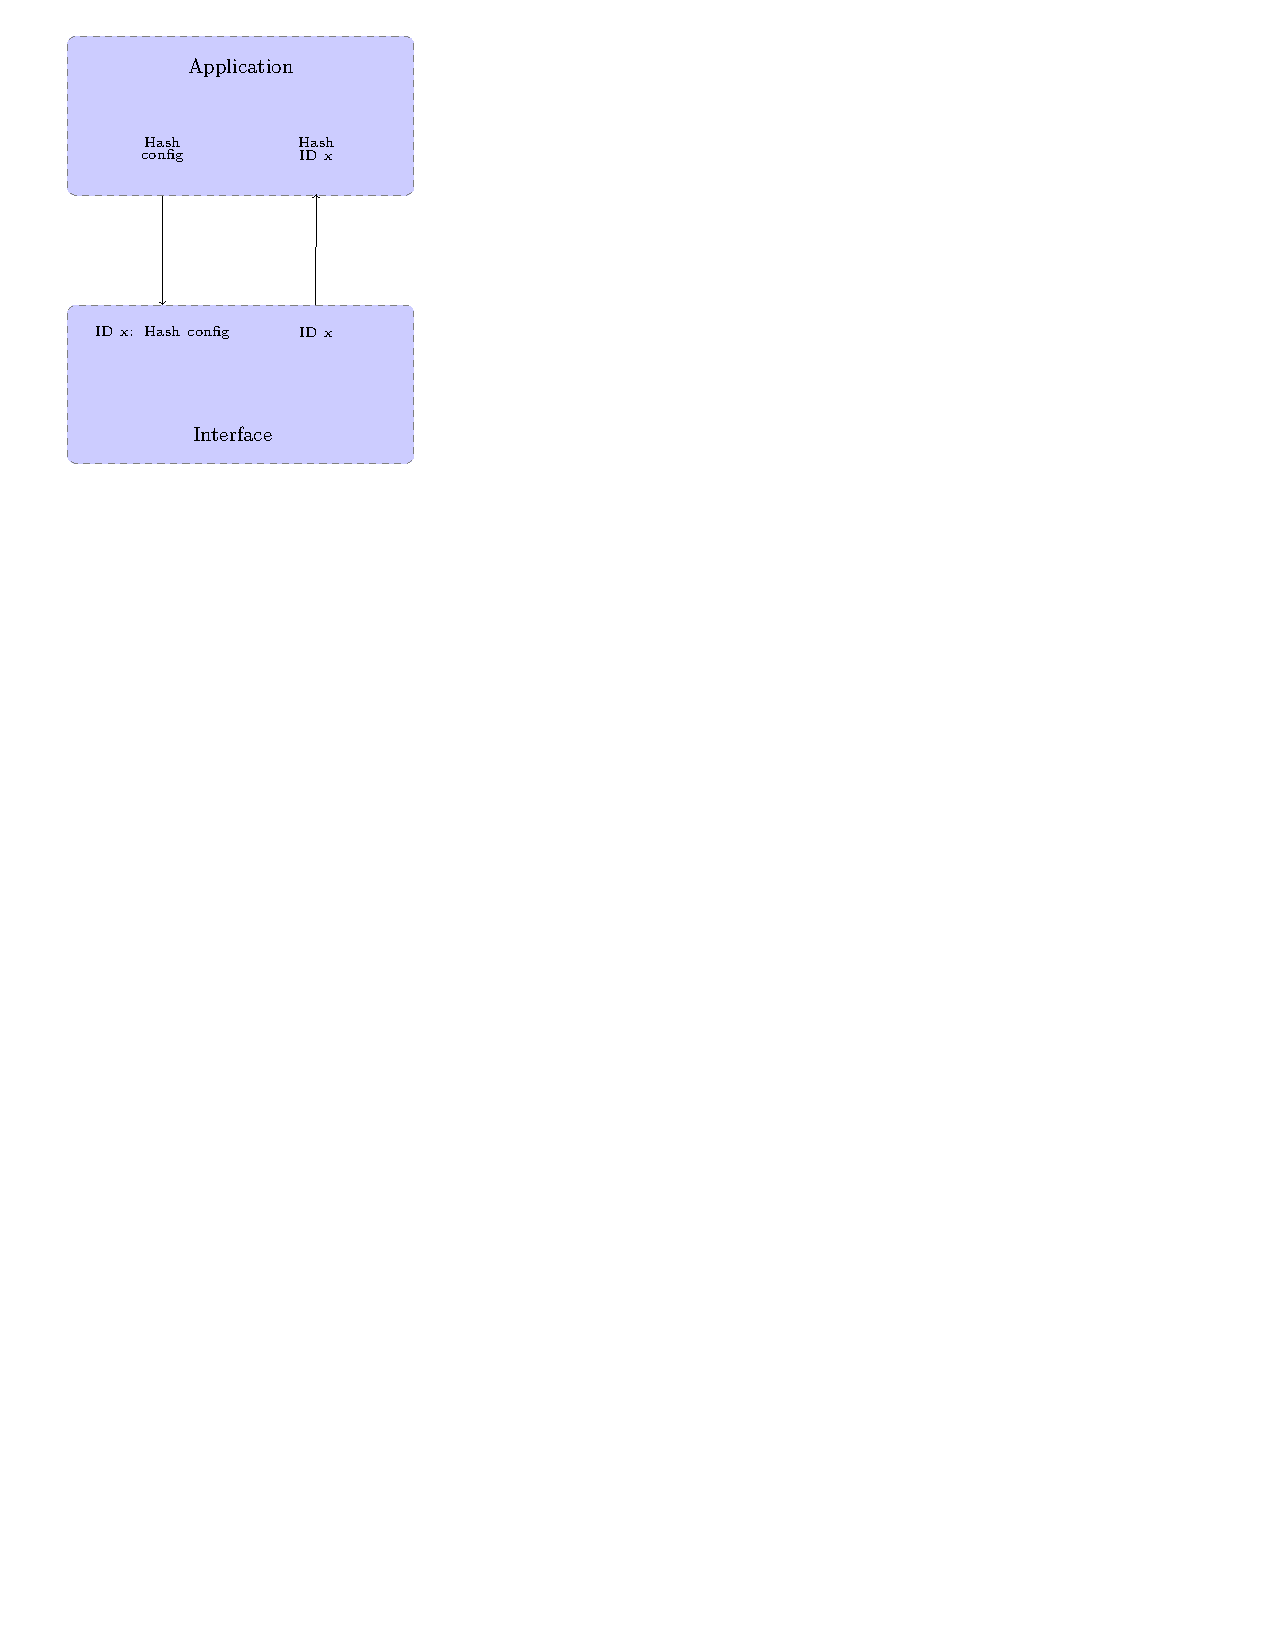
\includegraphics[trim=0cm 20cm 9.5cm 0cm]{figures/hash_example_config.pdf}
\caption{Hash - configuration\newline}
\label{fig:gci_hash_config}
%}
\end{figure}

When the configuration is done this one should be sent to the interface which
will save it in a context.
The interface will then return an ID of the context, which corresponds of
where is saved the configuration.
This is shown on figure \ref{fig:gci_hash_config} 

\subsection*{Update of data}

When the configuration is done, several updates can be done.
The principle on an update is to add a data which we want to hash.

\begin{figure}[!ht]
\centering
%\frame{
% trim: left, bottom, right, up
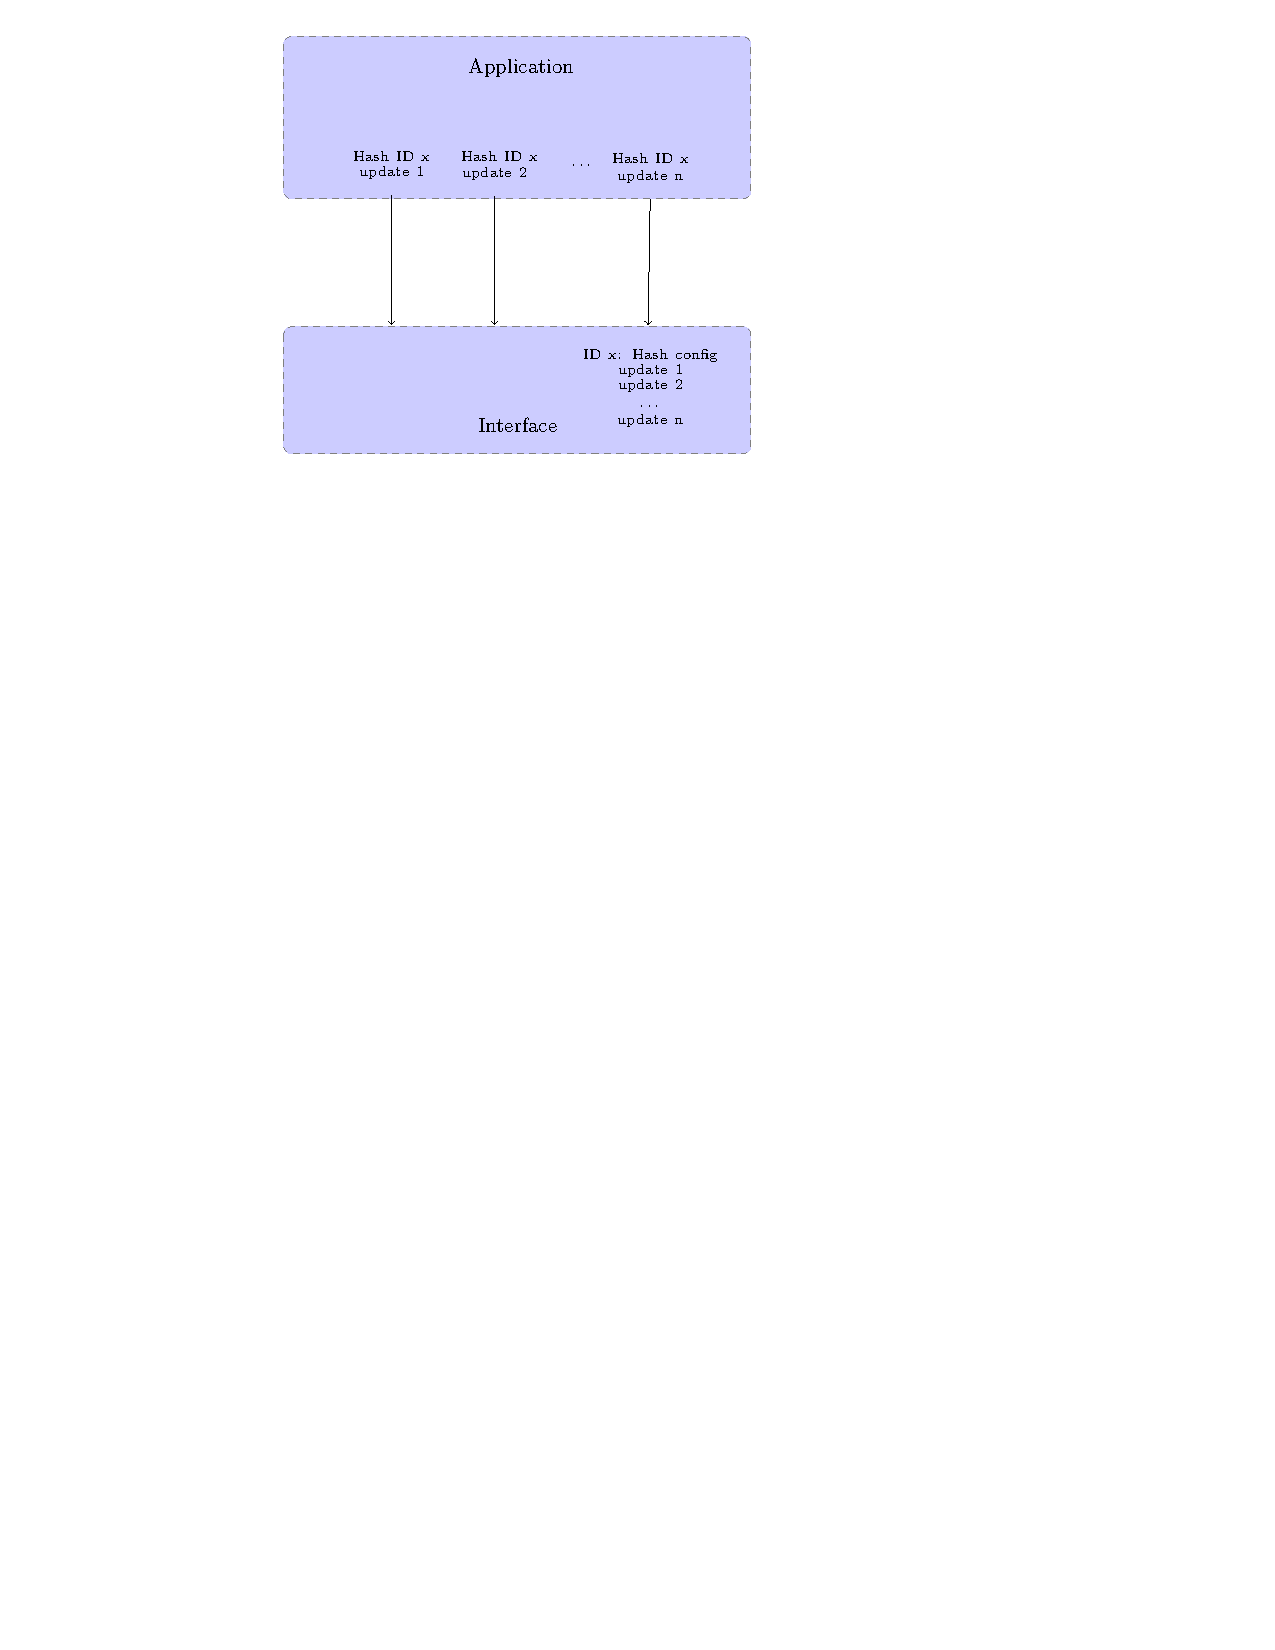
\includegraphics[trim=8cm 20cm 9.5cm 0cm]{figures/hash_example_update.pdf}
\caption{Hash - update\newline}
\label{fig:gci_hash_update}
%}
\end{figure}

As shown in the figure \ref{fig:gci_hash_update}, the ID received in the
configuration part has to be used to add a data.
The ID and the data has therefore sent to the interface, which knows through the
context ID that it should hash the data with the configuration saved in this
context.

\subsection*{Calculation of the digest}

When all the data we want to hash are sent to the interface, the interface can
calculate the digest.

\begin{figure}[!ht]
\centering
%\frame{
% trim: left, bottom, right, up
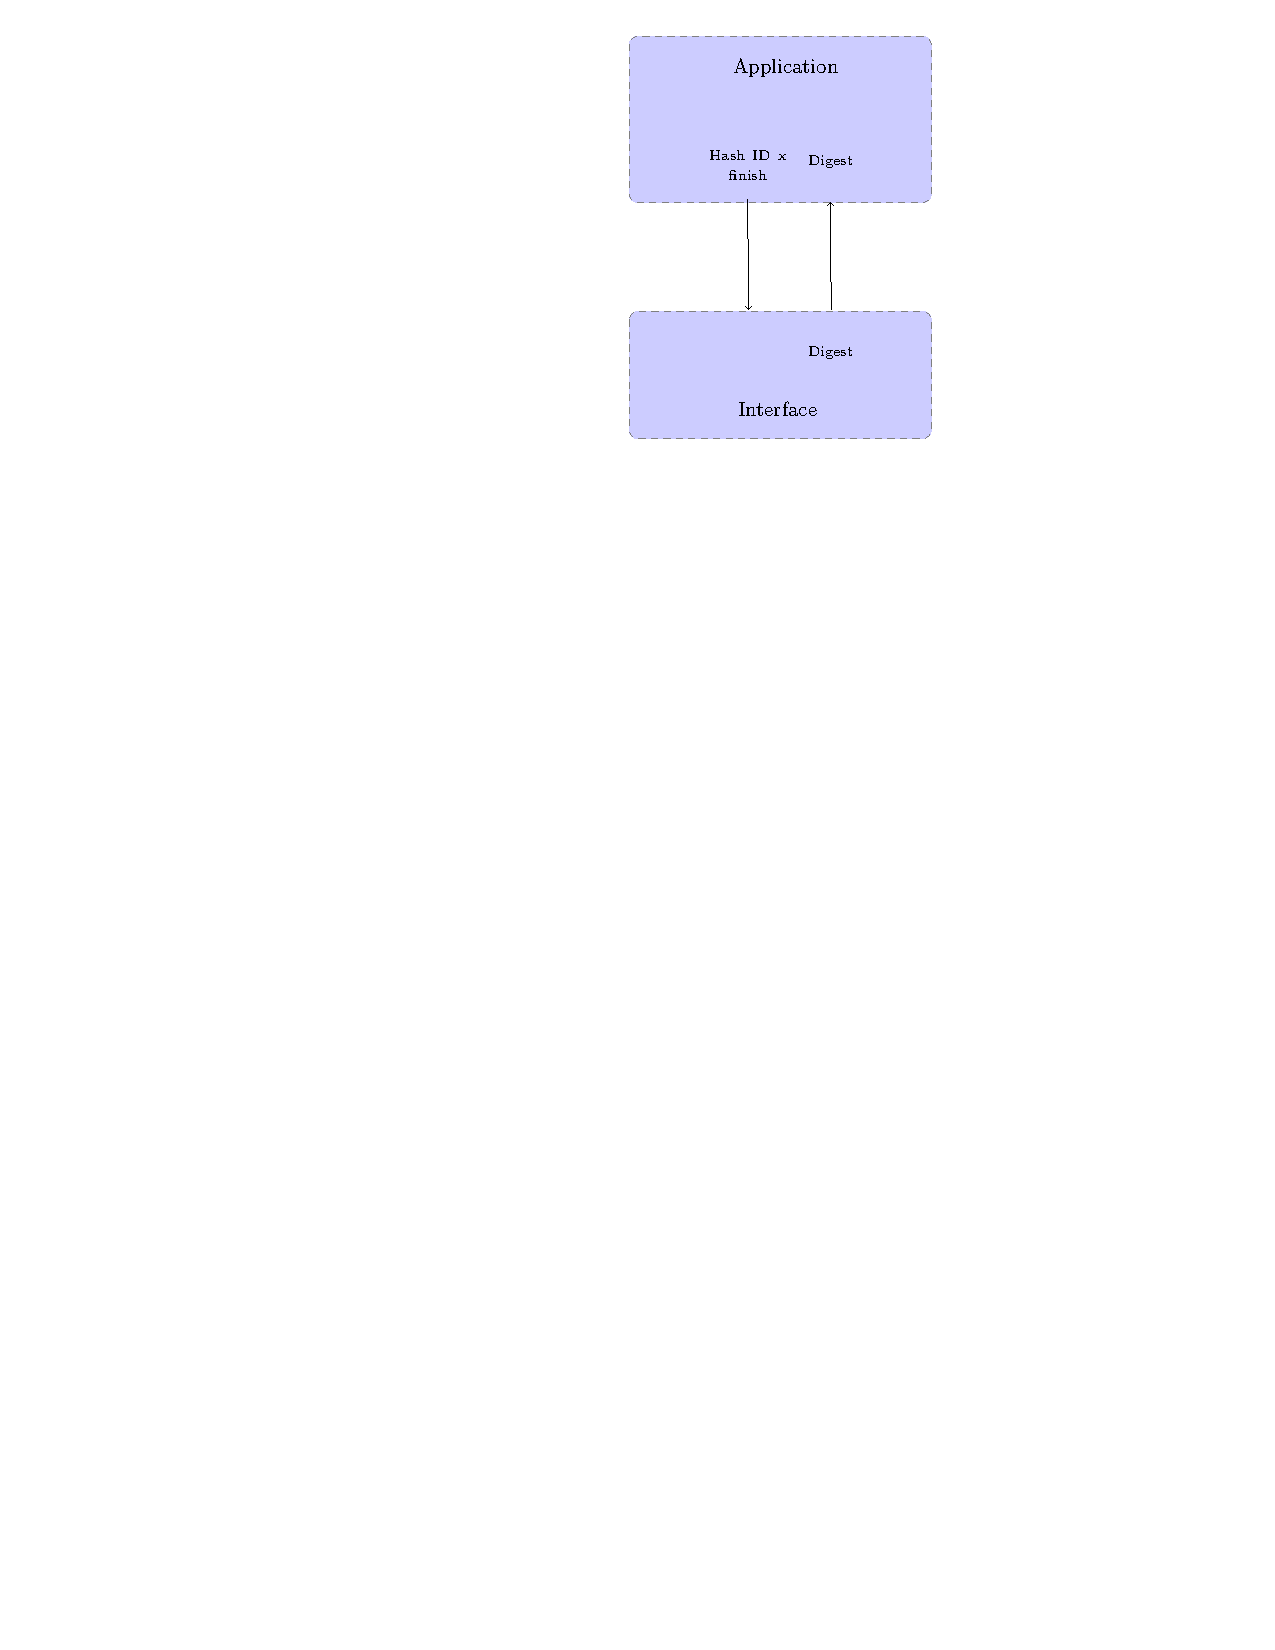
\includegraphics[trim=18.5cm 20cm 9.5cm 0cm]{figures/hash_example_finish.pdf}
\caption{Hash - finish\newline}
\label{fig:gci_hash_finish}
%}
\end{figure}

As shown in figure \ref{fig:gci_hash_finish}, by passing the ID which contains
the configuration and all the updated data, the interface will, through the
provider, calculate the digest.
One of the disadvantages of this part is
when the digest is calculated, all the updated data and the configuration are lost, meaning that we cannot use them
again to calculate another hash with other data.
This problem is solved in chapter \ref{gci_cl_ctx}

\subsection{Generate key pair}
\label{gci_gen_key}

Some parts of cryptography need keys to work, like signatures and ciphers.
The key can be a symmetric, which is the same key for the two peers
in a communication or asymmetric, which is different for the two peers in a
communication.
The goal of this function is to generate the asymmetric keys, public key and
private key. To generate a symmetric key, other methods should be used like
Diffie-Hellman.
In the interface, three kinds of key pair can be generated, each having a
different configuration:
\begin{itemize}
  \item RSA key pair\newline
  The size of the key should be configured (1024 bits, 2048 bits, 4096 bits,
  etc.)
  \item DSA key pair\newline
  The domain parameters can be configured if needed or internally generated
  \item ECDSA key pair (Elliptic curve)\newline
  The type of the elliptic curve should be configured
\end{itemize}

When the configuration is done, this one should be sent to the
interface.
The keys will then be generated through a cryptographic provider.
The keys are, however, returned as IDs, which is one of the principles of the
interface. For more details about the key ID see chapter key management
\ref{gci_key_mng}

\subsection{Digital signature - Message Authentication Code (MAC)}
\label{gci_sign_mac}

The digital signature and the MAC are widely used today. Both provide integrity
and authentication of a message. Only the digital signature provides
non-repudiation more. MAC is much faster than digital signature through the use
of symmetric keys.
As some specifications of certain provider, the signature/MAC function has two
possibilities of use:
\begin{enumerate}[noitemsep]
  \item Signing
  \item Verifying\newline
\end{enumerate}

Each one is split into three functions:
\begin{itemize}[noitemsep]
  \item Configuration of the signature
  \item Update of data
  \item Generate a signature/Verify a signature\newline
\end{itemize}


\subsection*{Configuration of the signature}
For the generation and verification of a signature this part is the same (only
the name of the function changes).
First should the signature be configured.
Several parameters have to be configured which are:
\begin{itemize}
  \item the signature/MAC algorithm, which could be:
  \begin{itemize}[noitemsep]
    \item RSA
    \item DSA
    \item ECDSA
    \item CMAC (MAC from Block Ciphers)
    \item HMAC (MAC from Hash functions)
  \end{itemize}
  \item A hash algorithm, if in the updated data should be first hashed before
  signing, or if the HMAC algorithm is used
  \item The padding, if the RSA algorithm is used
  \item The block mode, the padding and the initialization vector, if the CMAC
  algorithm is used
  \item The private key, if RSA, DSA or ECDSA is used to generate a signature or
  the public key if the same algorithm is used to verify a signature
\end{itemize}

\begin{figure}[!ht]
\centering
%\frame{
% trim: left, bottom, right, up
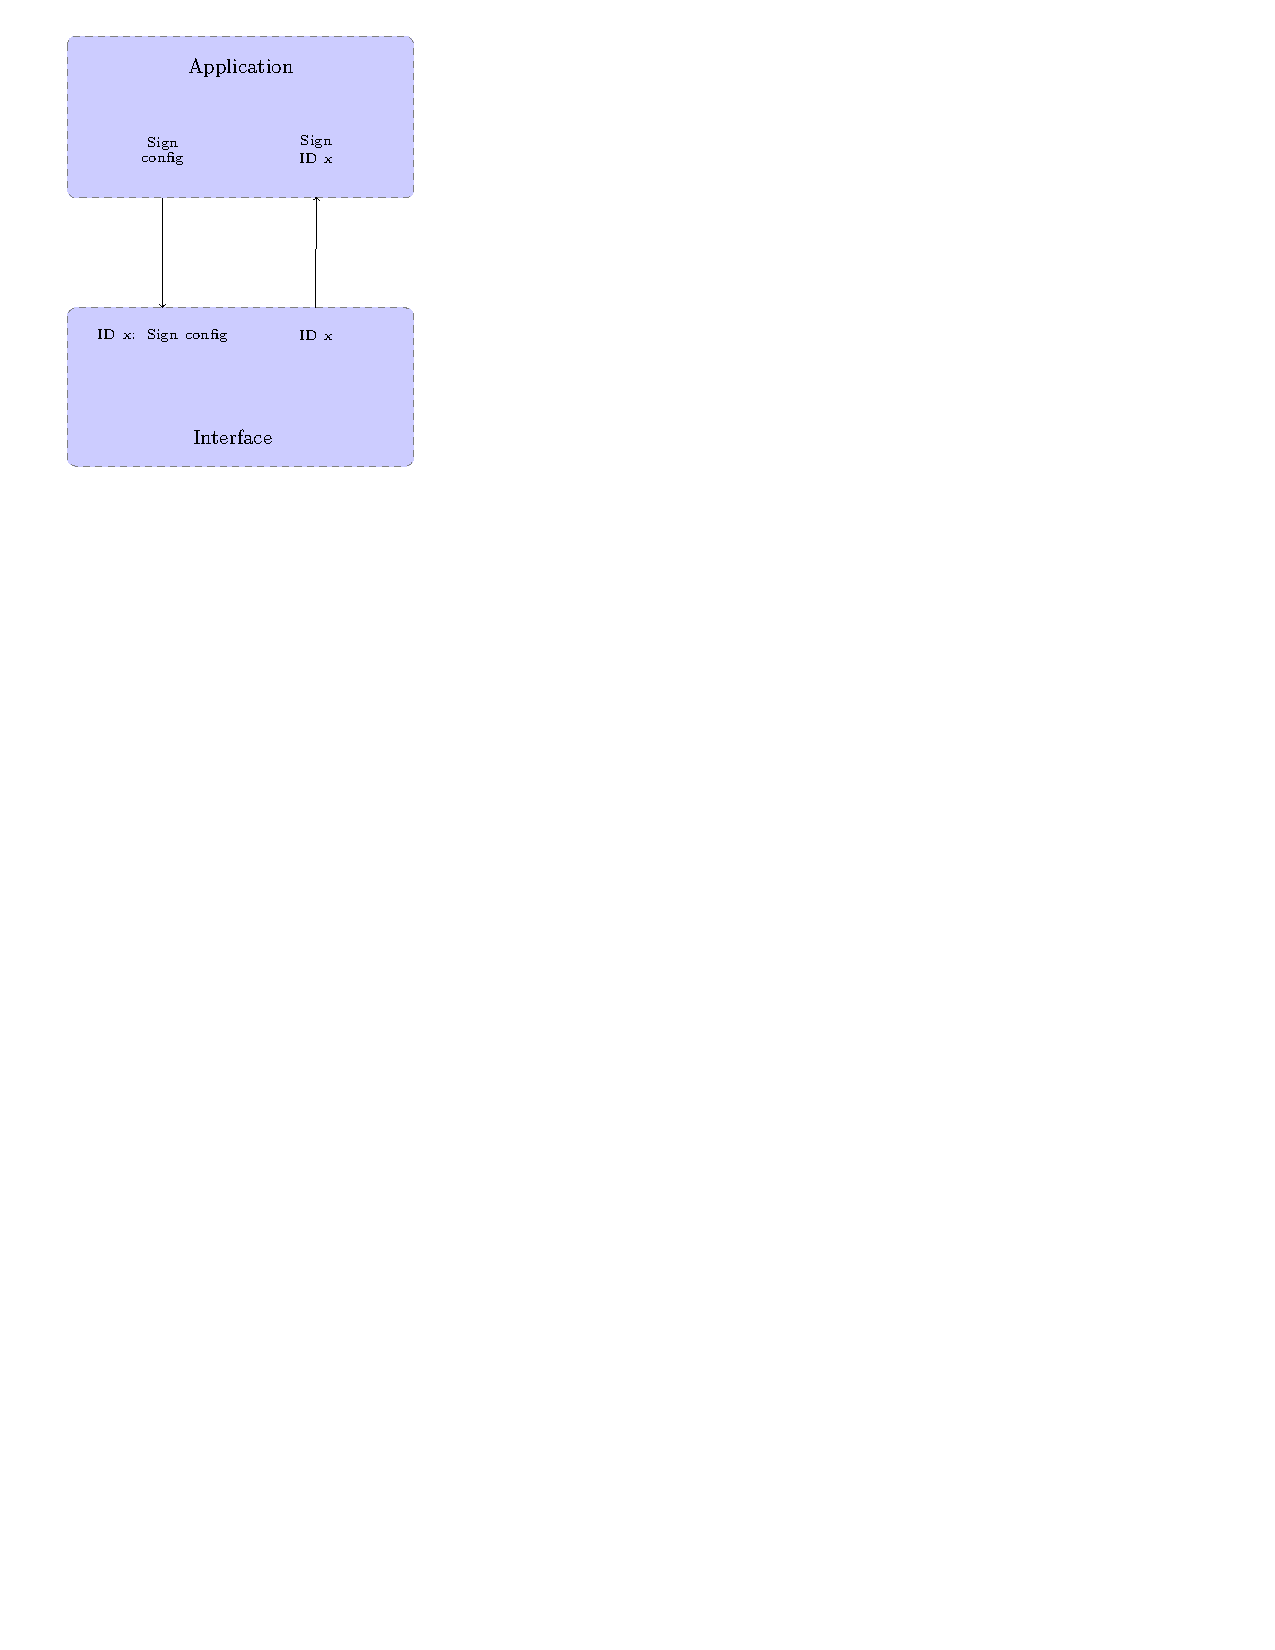
\includegraphics[trim=0cm 20cm 9.5cm 0cm]{figures/sign_example_config.pdf}
\caption{Signature - configuration\newline}
\label{fig:gci_sign_config}
%}
\end{figure}

As shown figure \ref{fig:gci_sign_config}, when the configuration is done, this
one is saved in a context in the interface. An ID of the context is returned,
which indicated where is the configuration saved.

\subsection*{Update of data} 

When the configuration is done, several updates could be done.\newline
The principle of the update is to add data which will be used to generate or
verify a signature.\newline

\begin{figure}[!ht]
\centering
%\frame{
% trim: left, bottom, right, up
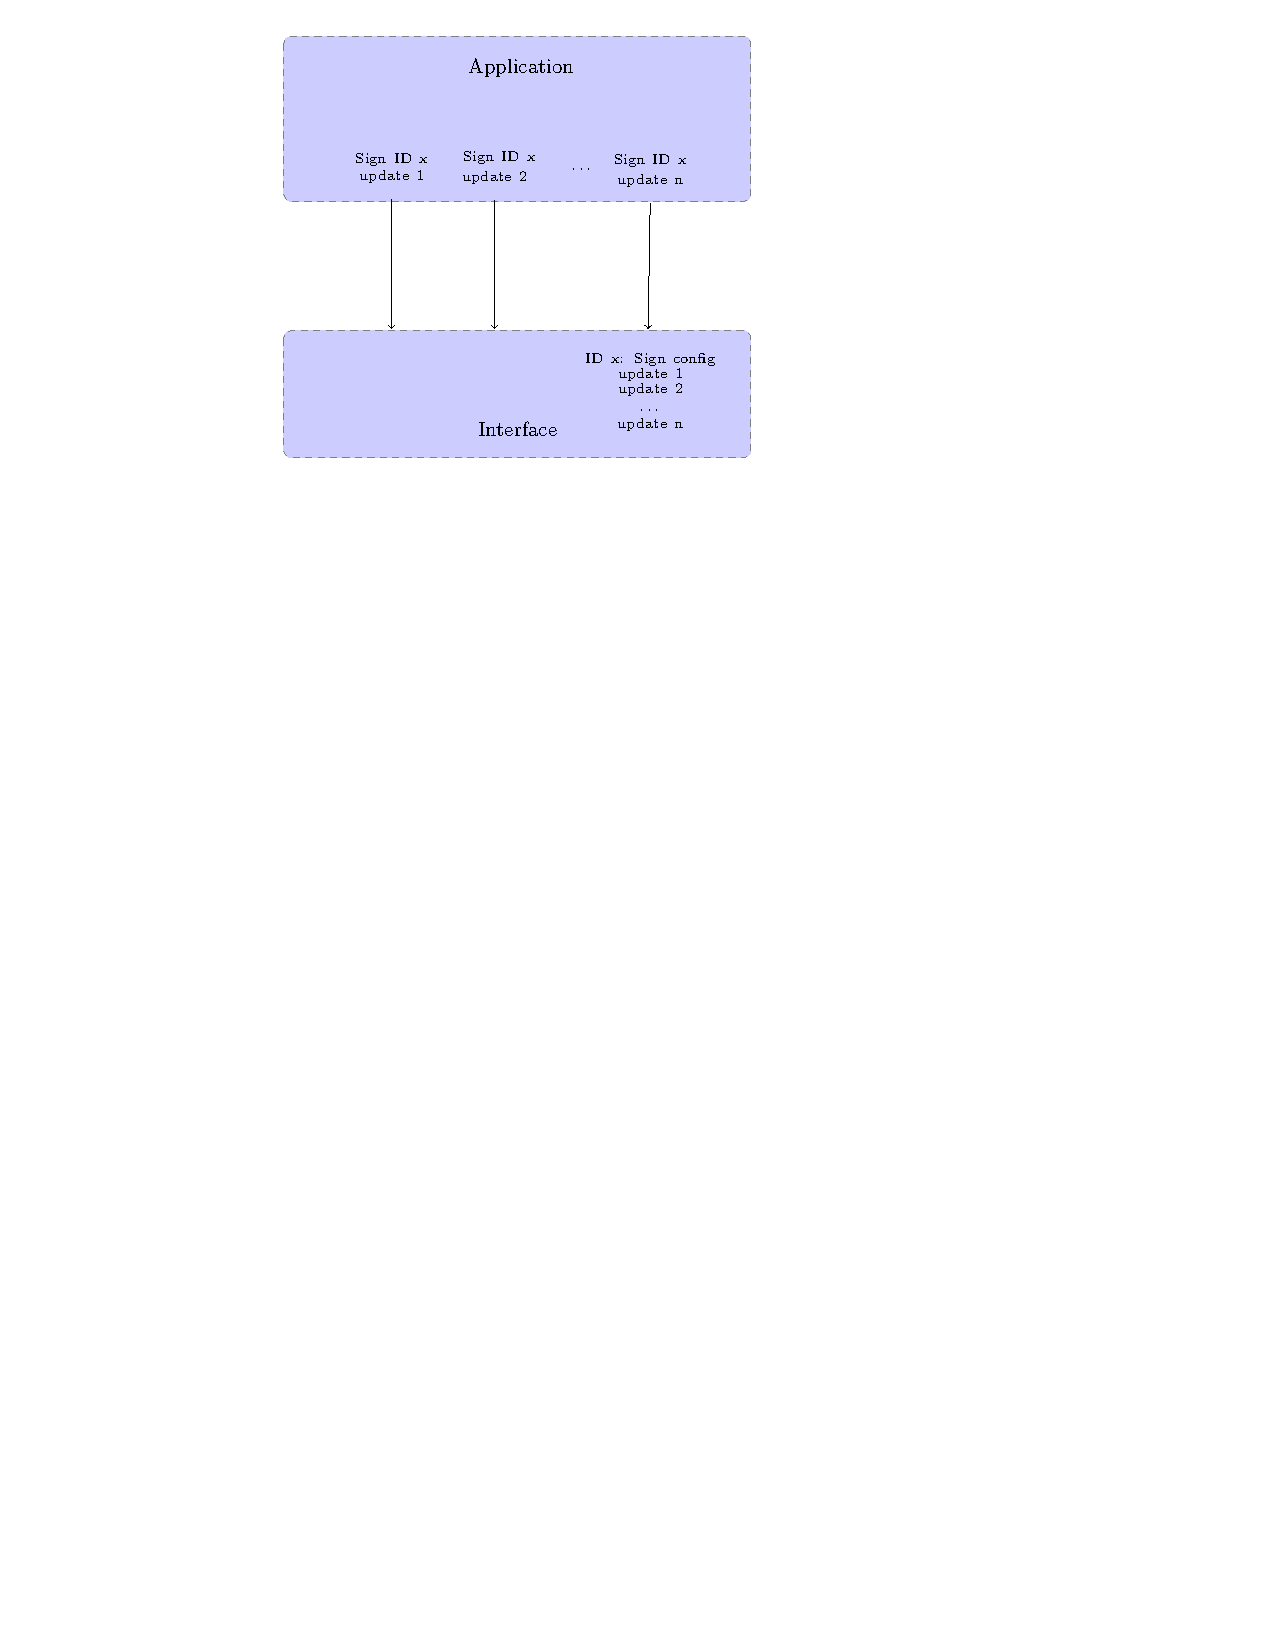
\includegraphics[trim=8cm 20cm 9.5cm 0cm]{figures/sign_example_update.pdf}
\caption{Signature - update\newline}
\label{fig:gci_sign_update}
%}
\end{figure}

As shown in figure \ref{fig:gci_sign_update}, to use the correct configuration,
the ID of the context, returned when the configuration is saved, should be
used.
The data and the ID is then sent to the interface, which will sign this data
with the configuration saved in this context.


\subsection*{Generate a signature/Verify a signature}
\begin{figure}[!ht]
\centering
%\frame{
% trim: left, bottom, right, up
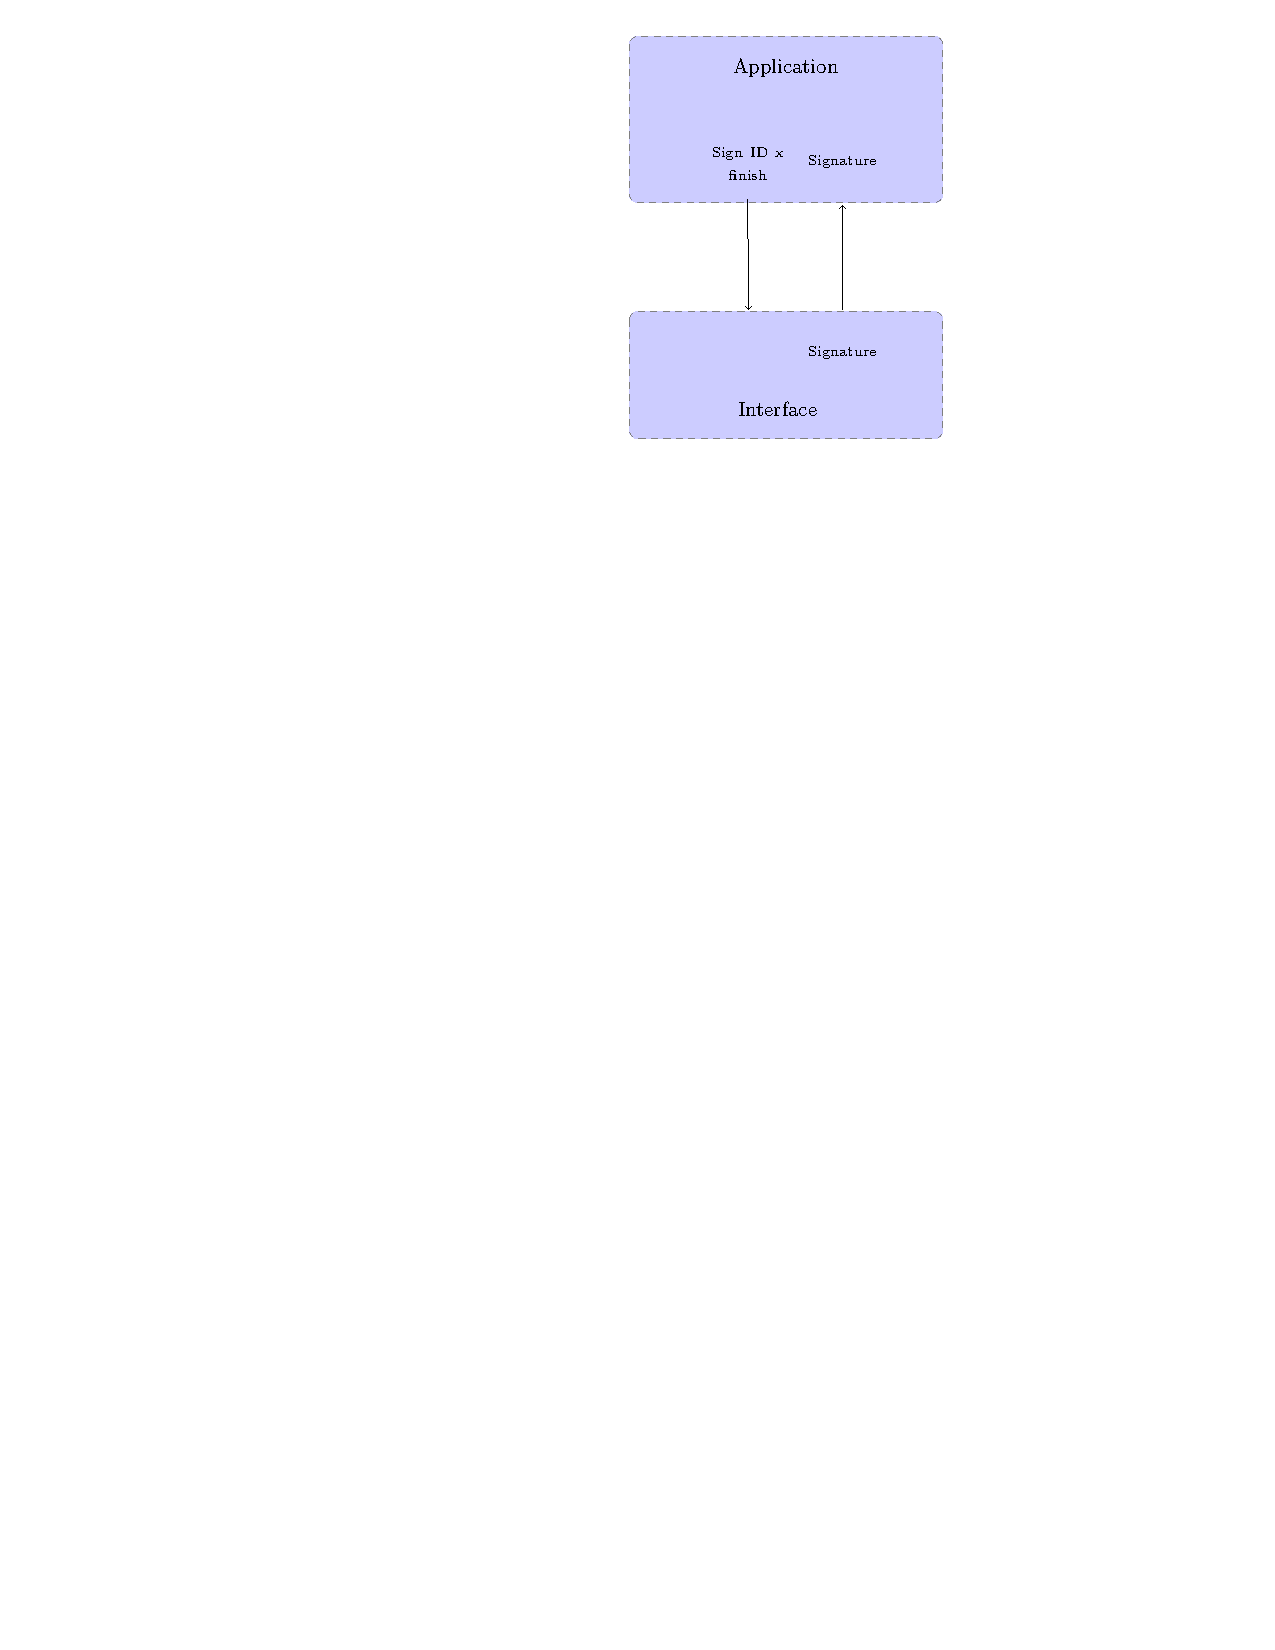
\includegraphics[trim=18.5cm 20cm 9.5cm 0cm]{figures/sign_example_finish.pdf}
\caption{Signature - finish\newline}
\label{fig:gci_sign_finish}
%}
\end{figure}
In this part the generation and the verification are different.
For the generation , the whole updated data and the configuration will be signed
with the private key added in the configuration for the digital
signature but with a symmetric key for the MAC.

For the verification, the signature we want to verify should be added to the
function.
Then the updated data will be signed, but with the public key for the
digital signature, and the same symmetric key as the generation of the
signature for the MAC.
Then the added signature (which is done with the
private key) could be compared with the ``signature'' computed to verify.
The most important part of the verification is that the private key, which
the signature is done and the public key for the verification, should be
generated together for the digital signature and the same symmetric key should
be used for the MAC.

\subsection{Cipher (symmetric and asymmetric)}
\label{gci_ciph}
A cipher, as explained in \ref{intro_cipher}, which
could be symmetric or asymmetric, is an algorithm for encrypting and decrypting
data.
This concept is therefore used in the interface and split into three main
functions which are:
\begin{itemize}[noitemsep]
  \item Configuration of the cipher
  \item Encryption of a plaintext
  \item Decryption of a ciphertext
\end{itemize}

\subsection*{Configuration of the cipher}
Several parameters are to be configured for the cipher algorithm and depends
particularly of which cipher algorithm is used.
The cipher algorithm is split into three main algorithm:

\begin{itemize}
  \item Symmetric stream cipher algorithm\newline
Today very deprecated but is, however, implemented in the interface if
comparison has to be done.
Only the RC4 stream cipher is implemented in the interface.
Other stream ciphers can, however, be easily added in the interface if
needed.
Nothing more as the algorithm has to be configured for the use of
it.
  \item Symmetric block cipher algorithm\newline
  Three kinds of symmetric block cipher algorithms are used today and
therefore implemented in the interface:
\begin{itemize}[noitemsep]
  \item Data Encryption Standard (DES)
  \item 3DES, three subsequent DES encryption
  \item Advanced Encryption Standard (AES)  
\end{itemize}
Each symmetric block cipher algorithm needs a mode of operation, named block
mode in the interface, which depends on the size of data we want to
encrypt.\newline
The block modes implemented in the interface are:
\begin{itemize}[noitemsep]
  \item Electronic Code Book mode (ECB)
  \item Cipher Block Chaining mode (CBC)
  \item Cipher Feedback mode (CFB)
  \item Output Feedback mode (OFB)
  \item Counter mode (CTR)
  \item Galois Counter Mode (GCM)
\end{itemize}
  \item Asymmetric algorithm\newline
  Only the RSA algorithm is implemented for this part of the interface.
  In practice to use the RSA algorithm this one should use a padding to increase
  the security of it.
  The best known padding in the Public-Key Cryptography Standard (PKCS) and is,
of course, implemented in the interface.\newline  
\end{itemize} 
The most important thing for a cipher is, of course, the key!
For a symmetric cipher, stream or block, the key is only a shared key.
For an asymmetric cipher, if an encryption will be done, a public key should
be added. If a decryption will be done, a private key should be added to the
configuration.

\begin{figure}[!ht]
\centering
%\frame{
% trim: left, bottom, right, up
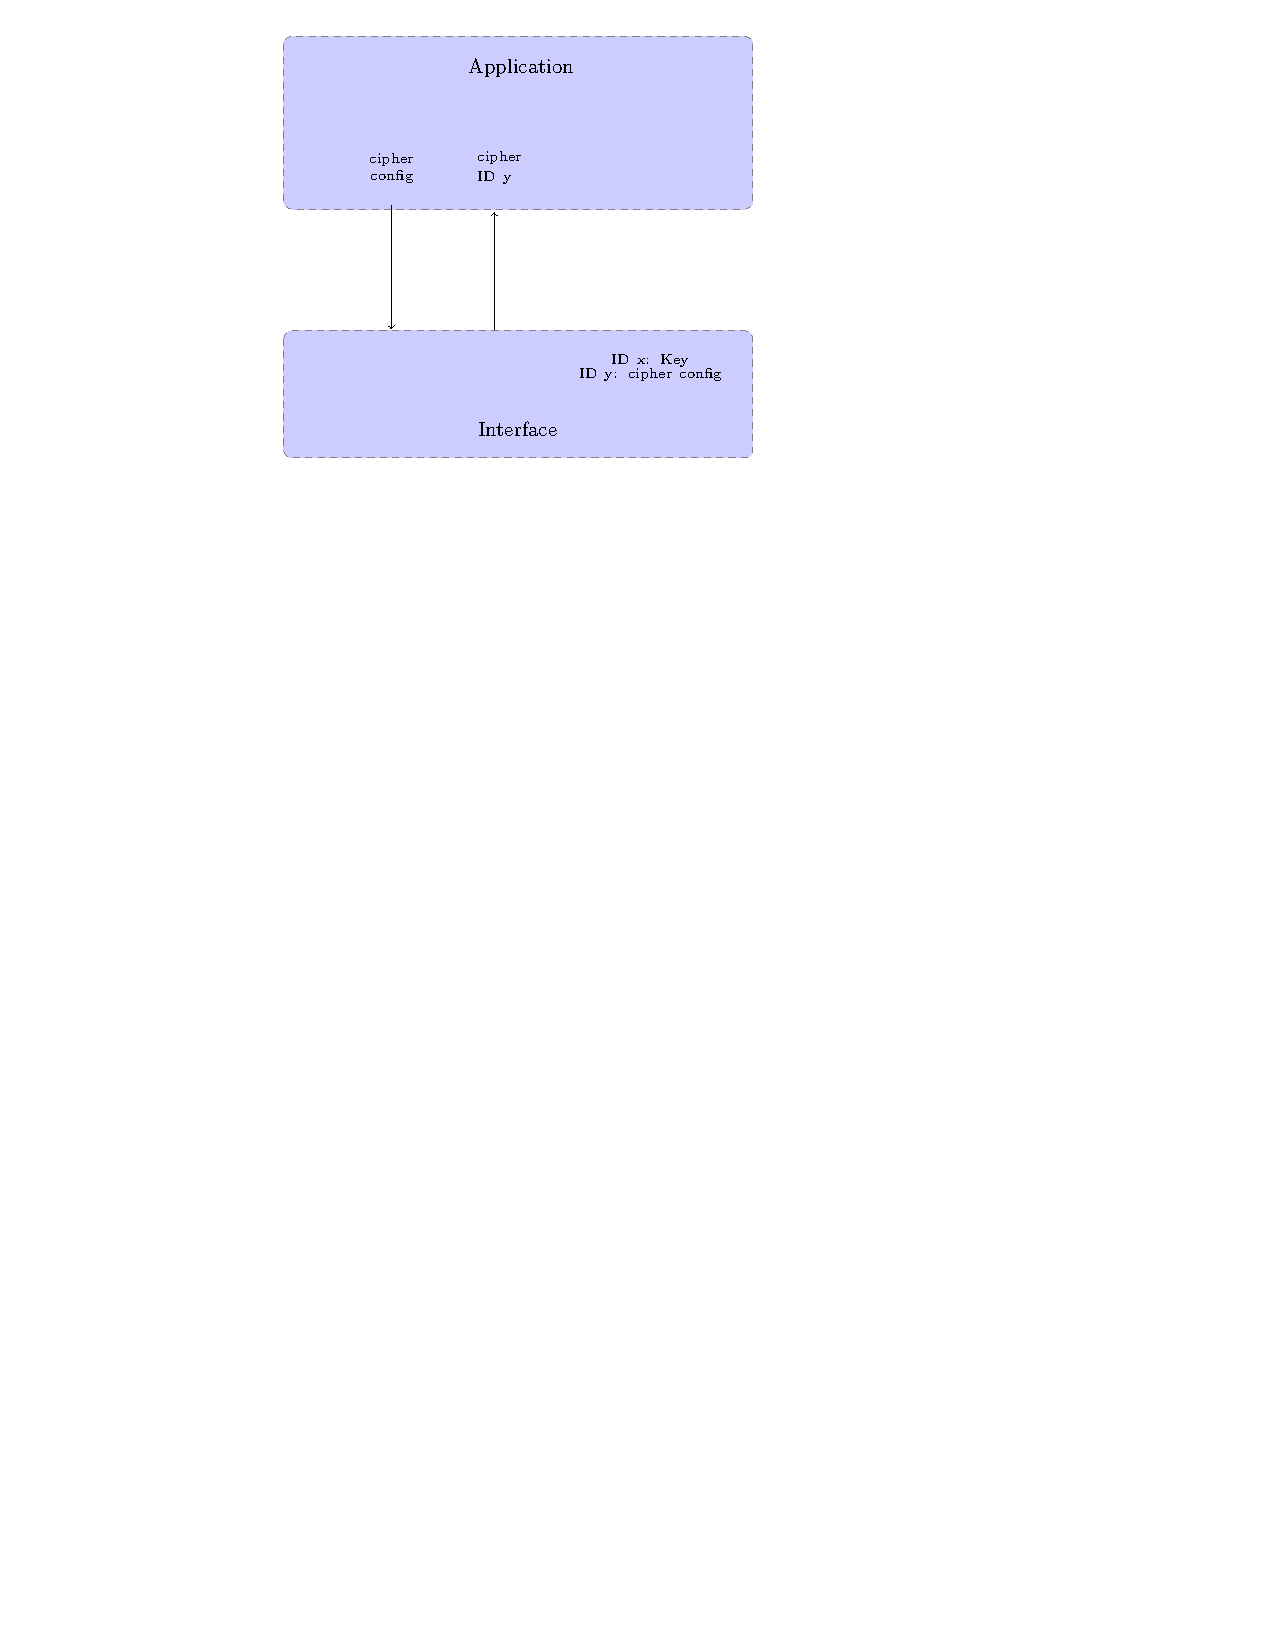
\includegraphics[trim=8.5cm 20cm 9.5cm 0cm]{figures/cipher_example_config.pdf}
\caption{Cipher - configuration\newline}
\label{fig:gci_cipher_config}
%}
\end{figure}

When the configuration is done this one should be sent to the interface
which will save it in a context.
The interface returned an ID of the context, which corresponds of where is saved
the configuration if this one should be used in the future.
The key added to the function is an ID of the key which is already saved in
the interface.
This principle is shown in figure \ref{fig:gci_cipher_config}

\subsection*{Encryption of a plaintext}
\begin{figure}[!ht]
\centering
%\frame{
% trim: left, bottom, right, up
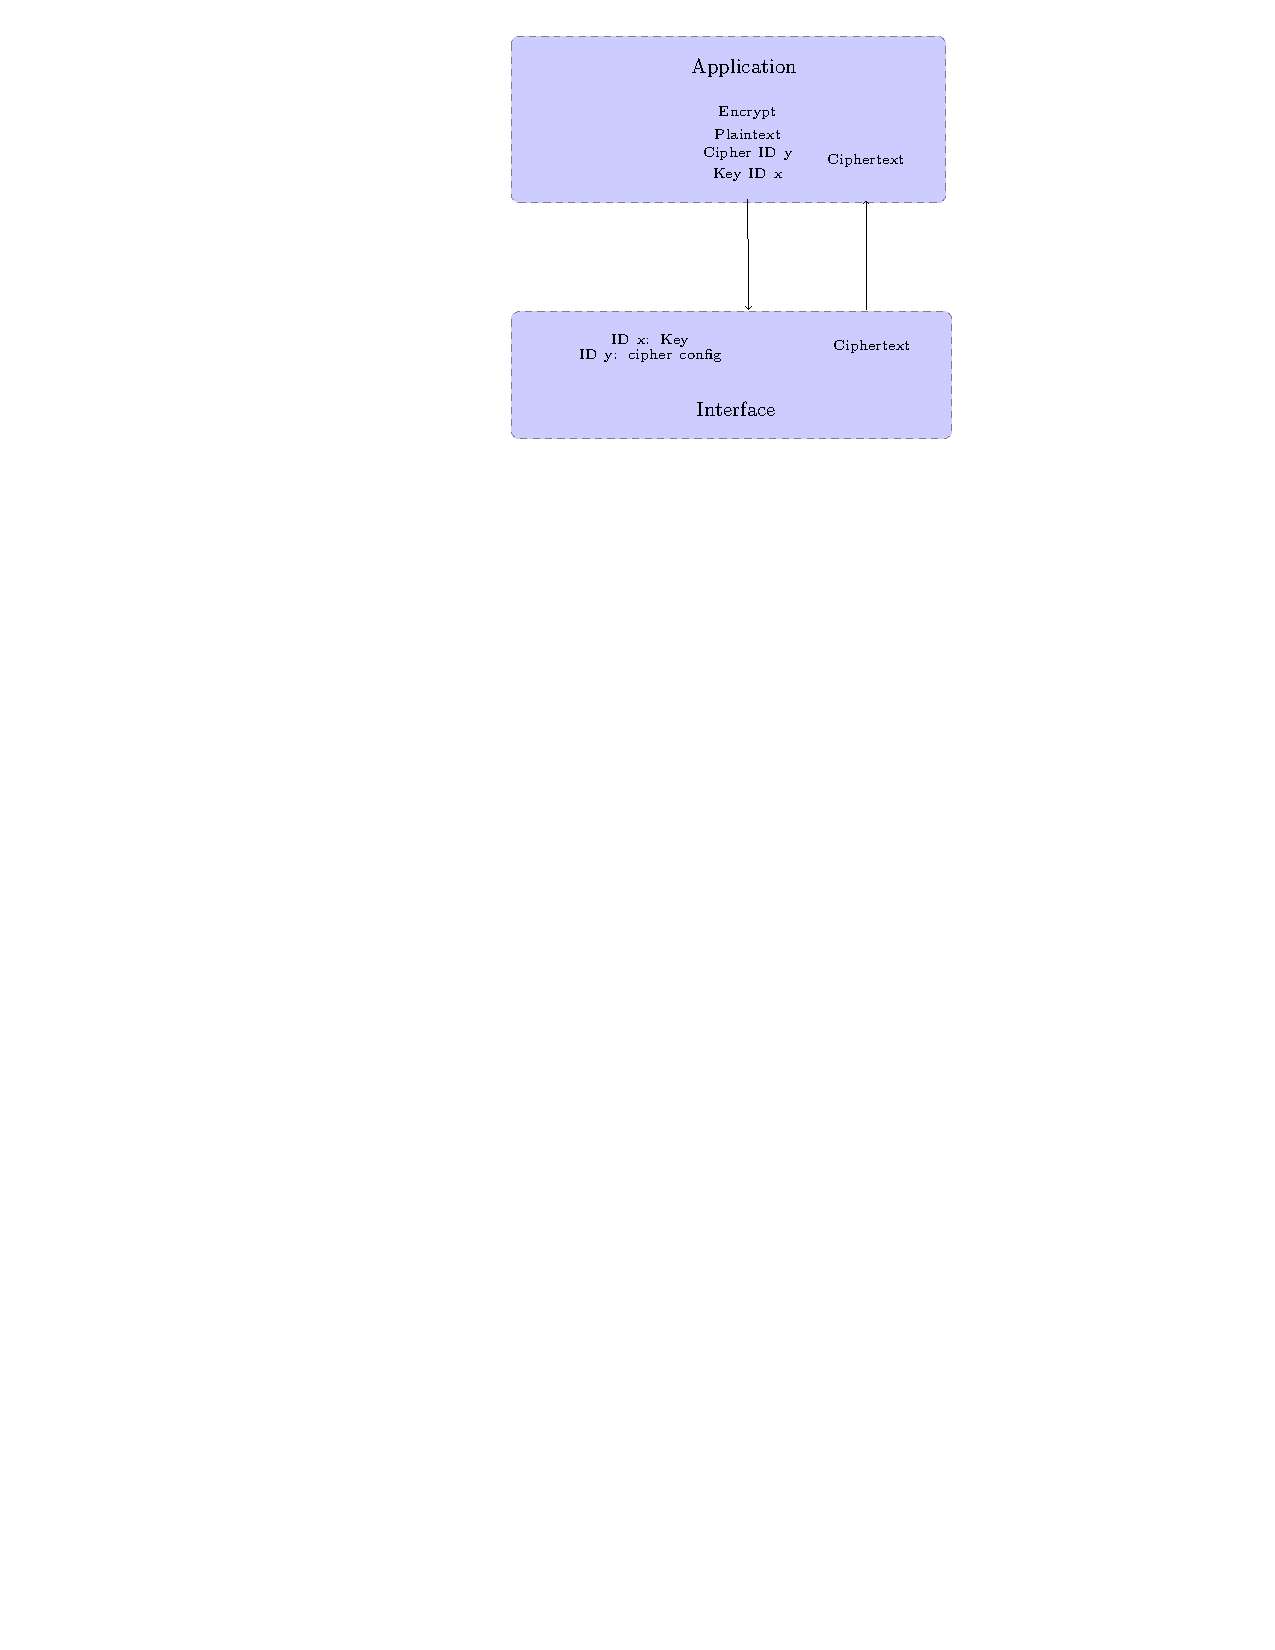
\includegraphics[trim=16cm 20cm 9.5cm 0cm]{figures/cipher_encrypt.pdf}
\caption{Cipher - Encryption\newline}
\label{fig:gci_cipher_encrypt}
%}
\end{figure}
When the configuration is done, a encryption can be done.
To encrypt data, the ID of the context (where is the configuration saved)
should be added to the function with the data to encrypt (plaintext).
The interface will, through a provider, calculate the ciphertext of the
plaintext with the configuration saved previously in the context.
This principle is shown figure \ref{fig:gci_cipher_encrypt}


\subsection*{Decryption of a ciphertext}

\begin{figure}[!ht]
\centering
%\frame{
% trim: left, bottom, right, up
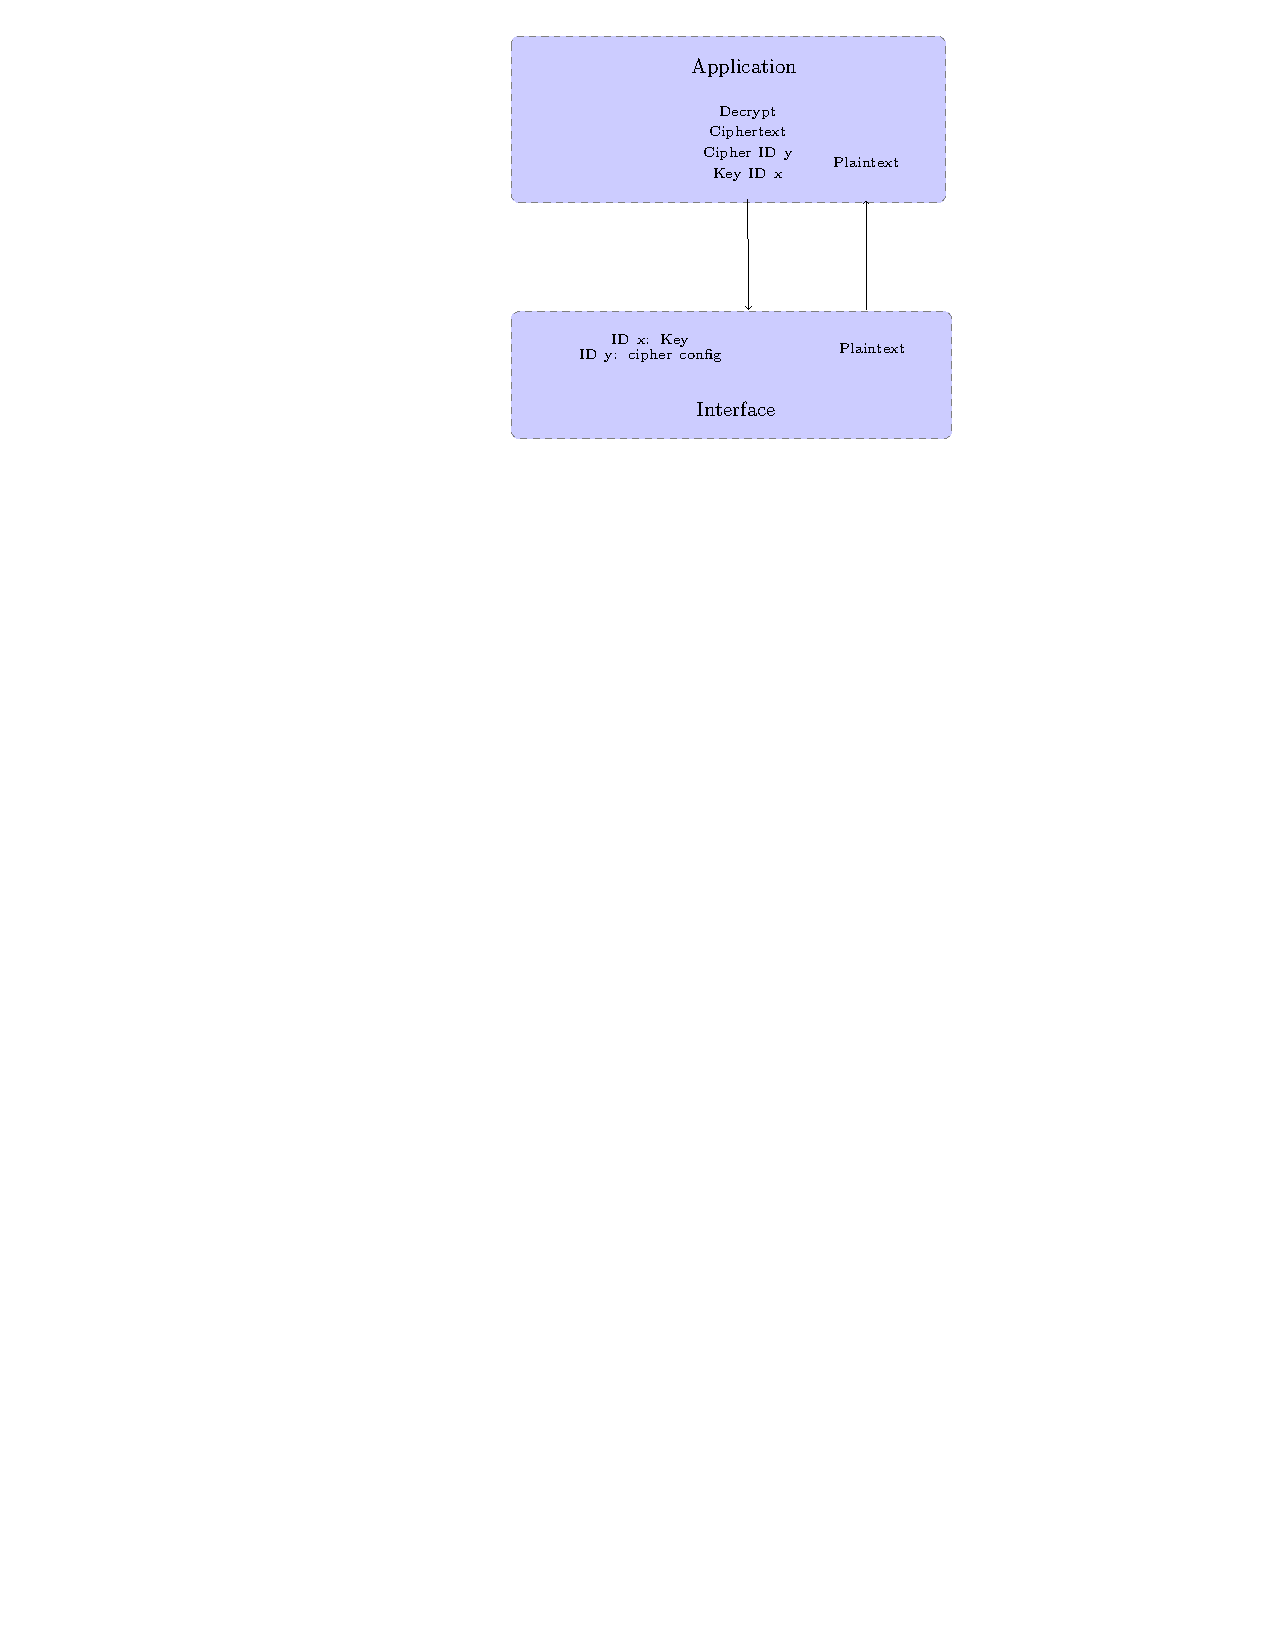
\includegraphics[trim=16cm 20cm 9.5cm 0cm]{figures/cipher_decrypt.pdf}
\caption{Cipher - Decryption\newline}
\label{fig:gci_cipher_decrypt}
%}
\end{figure}
When the configuration is done, a decryption can be done.
To decrypt a data, the ID of the context (where is the configuration saved)
should be added to the function with the data to decrypt (ciphertext).
The interface will, through a provider, calculate the plaintext of the
ciphertext with the configuration saved previously in the context.
This principle is shown figure \ref{fig:gci_cipher_decrypt}


\subsection{Diffie-Hellman}
\label{gci_dh}

Diffie-Hellman key exchange is a specific method of securely exchanging
cryptographic keys over an insecure network. It starts with asymmetric keys to finish with a
symmetric, shared key which is the same for the two peer in a communication.

The Diffie-Hellman key exchange should therefore have the possibility to
generate key pairs and to calculate the shared key.

That's why in the interface the Diffie-Hellman protocol is split into three main
functions:
\begin{itemize}[noitemsep]
  \item Configuration of the Diffie-Hellman protocol
  \item Generation key pair
  \item Calculation of the shared key
\end{itemize}


\subsubsection*{Configuration of the Diffie-Hellman protocol}
The Diffie-Hellman key exchange and the Elliptic Curve of Diffie-Hellman key
exchange can be used in the interface.
For the configuration, one of these key exchanges should be chosen.

For the Diffie-Hellman key exchange the domain parameters can be added. If no
domain parameters have been added, the interface will, through the provider,
generate them.

For the Elliptic Curve of Diffie-Hellman key exchange, the type of curve should
be configured.

\begin{figure}[!ht]
\centering
%\frame{
% trim: left, bottom, right, up
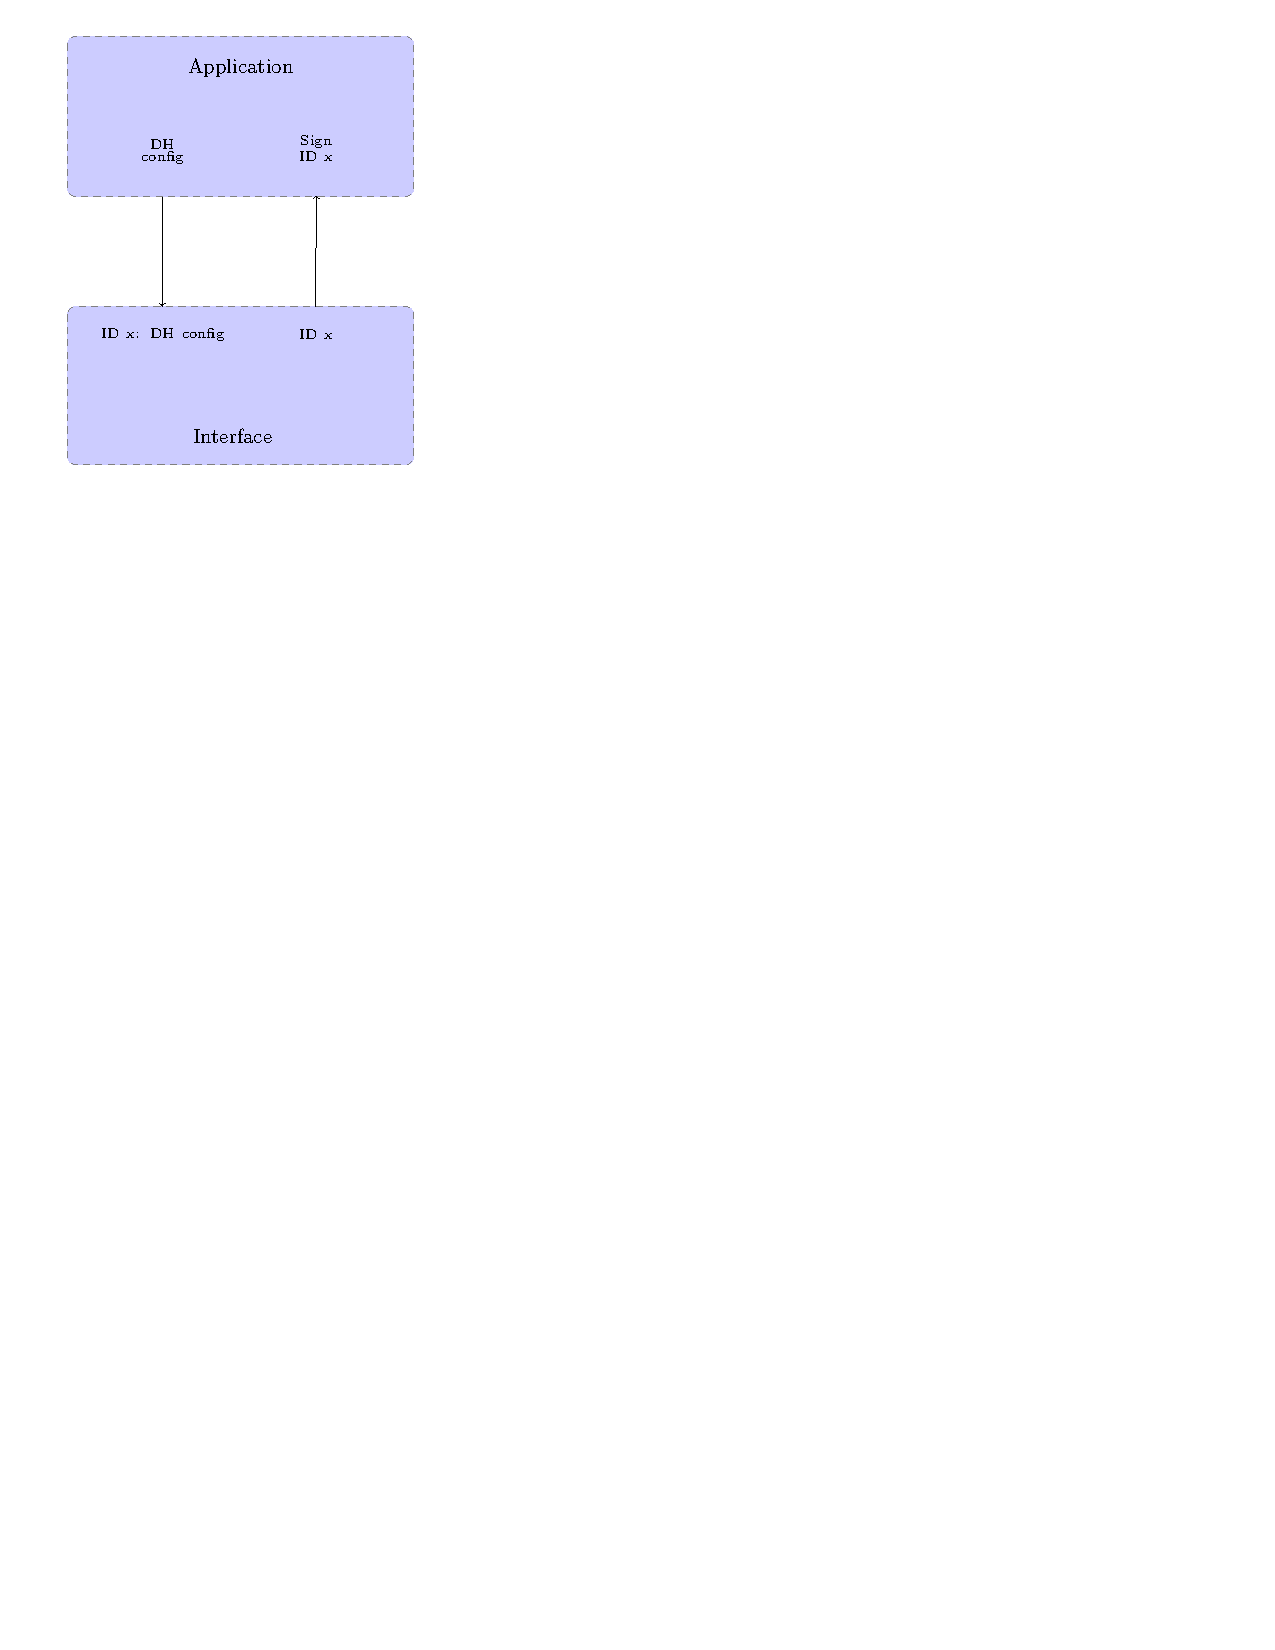
\includegraphics[trim=0cm 20cm 10cm 0cm]{figures/gci_dh_config.pdf}
\caption{DH - Configuration\newline}
\label{fig:gci_dh_config}
%}
\end{figure}

As shown on figure \ref{fig:gci_dh_config}, when the configuration is done, this
one should be sent to the interface which will save it in a context.
An ID of the context will be returned to the application, which indicates the
placement of the context, also of the configuration.


\subsubsection*{Generation of the key pair}

When the configuration is done, key pair can be generated. It's the same
principle as explain in the chapter \ref{gci_gen_key}, but for the
Diffie-Hellman it's a little bit different. The private key of the Diffie must not go out of the
interface. That's why when the key should be generated only the ID of the public
key will go out of the function. The private key will be saved in the
context, same context where is the configuration saved. This is why
Diffie-Hellman is not implemented with the asymmetric cipher algorithm, where
the public key and private key are going out of the function and don't stay in
the context. This is shown on figure \ref{fig:gci_dh_gen_key}

\begin{figure}[!ht]
\centering
%\frame{
% trim: left, bottom, right, up
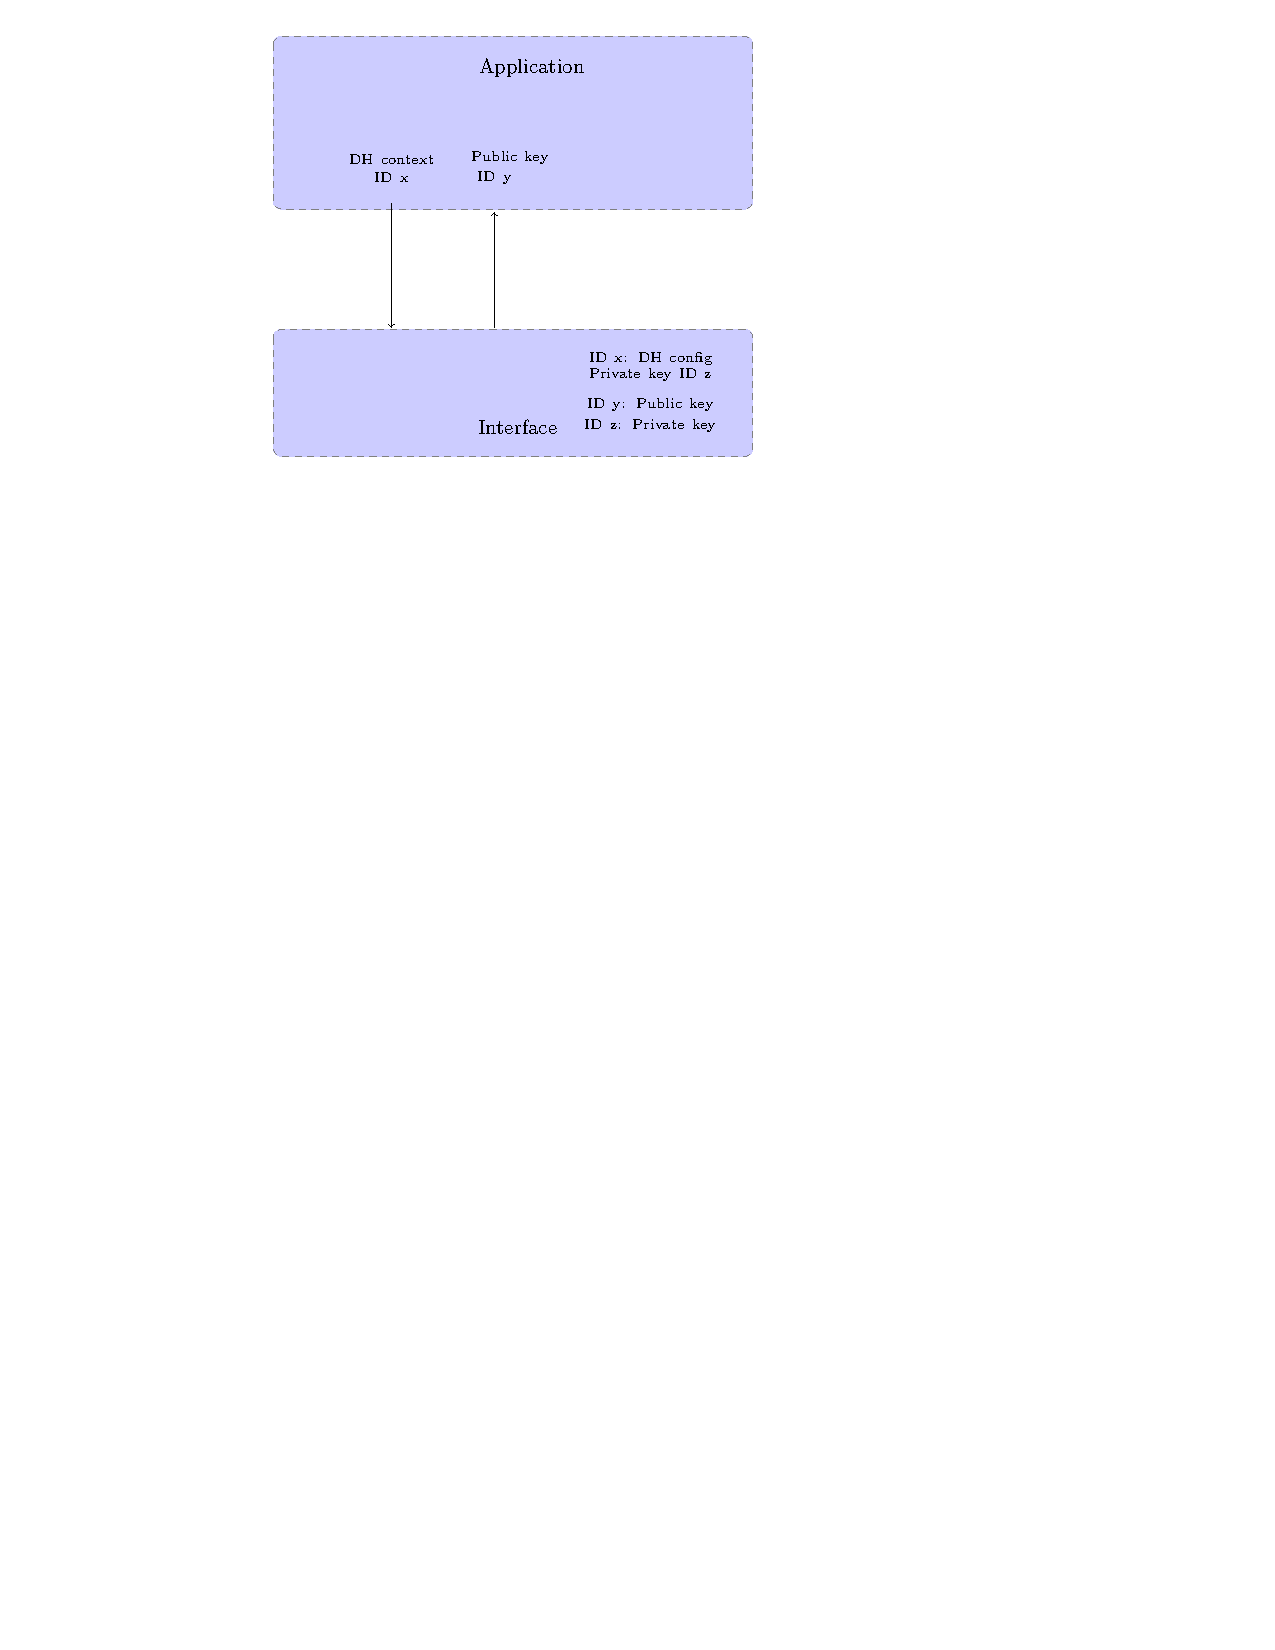
\includegraphics[trim=8.5cm 20cm 10cm 0cm]{figures/gci_dh_gen_key.pdf}
\caption{Diffie-Hellman - Generate key pair\newline}
\label{fig:gci_dh_gen_key}
%}
\end{figure}


\subsubsection*{Calculation of the shared key}

When the public key of the peer is received, the shared key could be generated.
To do it, the context with the configuration and the private, and the public key
of the peer should be added to the interface. This one will, through a provider
calculate the shared key and returned the ID of this one. This is shown on
figure \ref{fig:gci_dh_calc_key}

\begin{figure}[!ht]
\centering
%\frame{
% trim: left, bottom, right, up
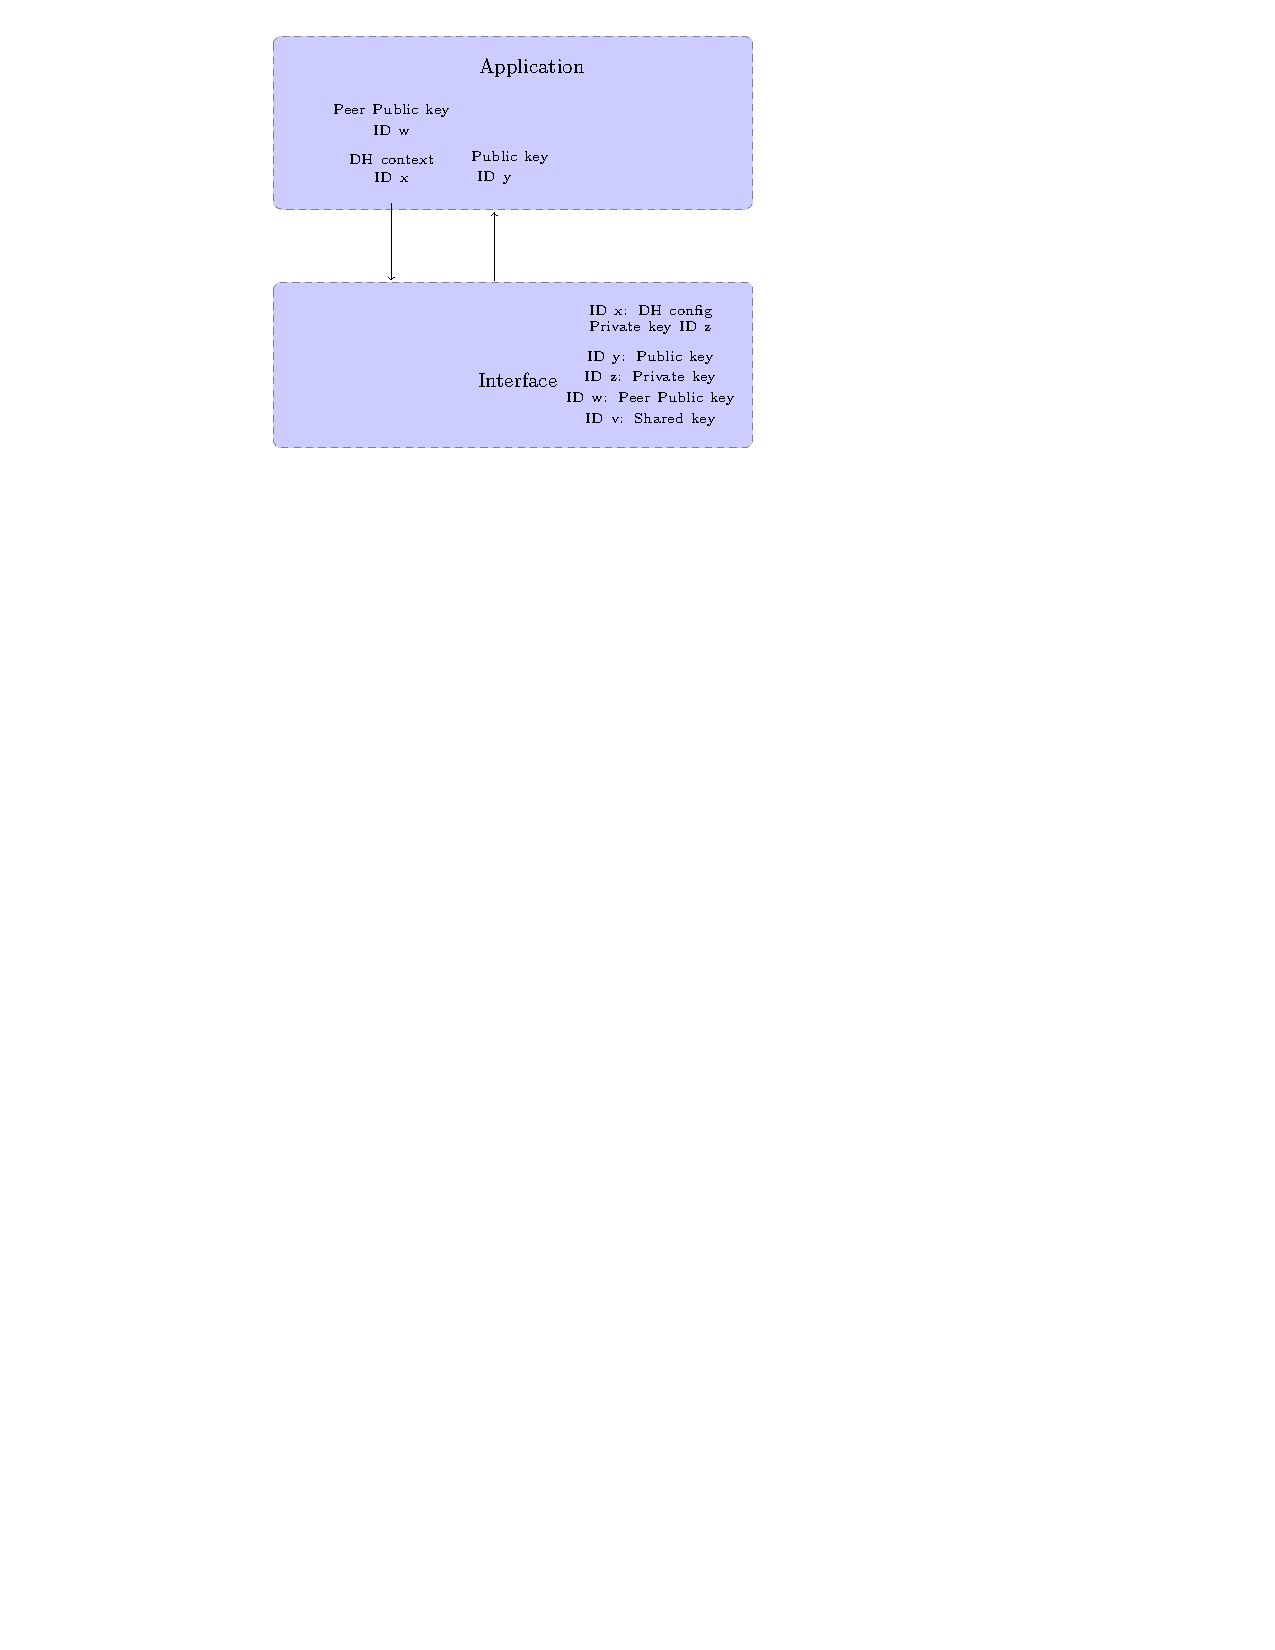
\includegraphics[trim=8.5cm 20cm 10cm 0cm]{figures/gci_dh_calc_key.pdf}
\caption{Diffie-Hellman - Calculation of the shared key\newline}
\label{fig:gci_dh_calc_key}
%}
\end{figure}


\subsection{Random number generator}
\label{gci_rng}

A random number generator is a computational or physical devices for generating
a sequence of numbers which are impossible to predict better than a random
chance.\newline
It exists two main random number generator:
\begin{enumerate}
  \item True Random Number Generators (TRNG)\newline
  Are characterized that the output cannot be reproduced. They are based on
  physical processes like semiconductor noise or clock jitter in digital
  circuits, etc..
  \item Pseudorandom Number Generators (PNRG)
  Generated sequences which are computed from an initial seed value. PRNGs
  possess good static properties, meaning their output approximates a sequence
  of true random numbers. This is shown on figure \ref{fig:gci_prng}
\end{enumerate}

For the interface, Random number generators are very important, to generate keys
or for the ciphers, for example.

For the use of a True Random Number Generator (TRNG), with hardware-based
cryptographic modules for example, only the function to get a random number is
needed.

For the use of Pseudo Random Number Generator (PRNG), with a
cryptographic software library for example, a function to generate the initial
seed value is, furthermore, needed.


\section{Clone of context}
\label{gci_cl_ctx}
As explained in \ref{gci_hash} and \ref{gci_sign_mac} when the digest (for the hash)
and the signature (for the digital signature/MAC) is calculated, no more data
can be added to the context.
This is a problem for the use of this interface in TLS projects (\embtls for
example).
Several solutions were introduced which are:
\begin{enumerate}
  \item Use two contexts at the same time.\newline
  This wasn't very efficient, because we should know at the beginning the
  number of times a digest will be calculated, which determines the amount of
  context we have to create at the beginning.
  \item Create a context when the digest is calculated.\newline
  The disadvantage of this idea was that the whole data use previously has to be
  saved. For applications, which are used in embedded systems, like \embtls, For
  systems, like embedded systems, with memory constraints, this is not possible.
  \item Clone the context. This is the solution uses for the interface.\newline
\end{enumerate}
\begin{figure}[!ht]
\centering
%\frame{
% trim: left, bottom, right, up
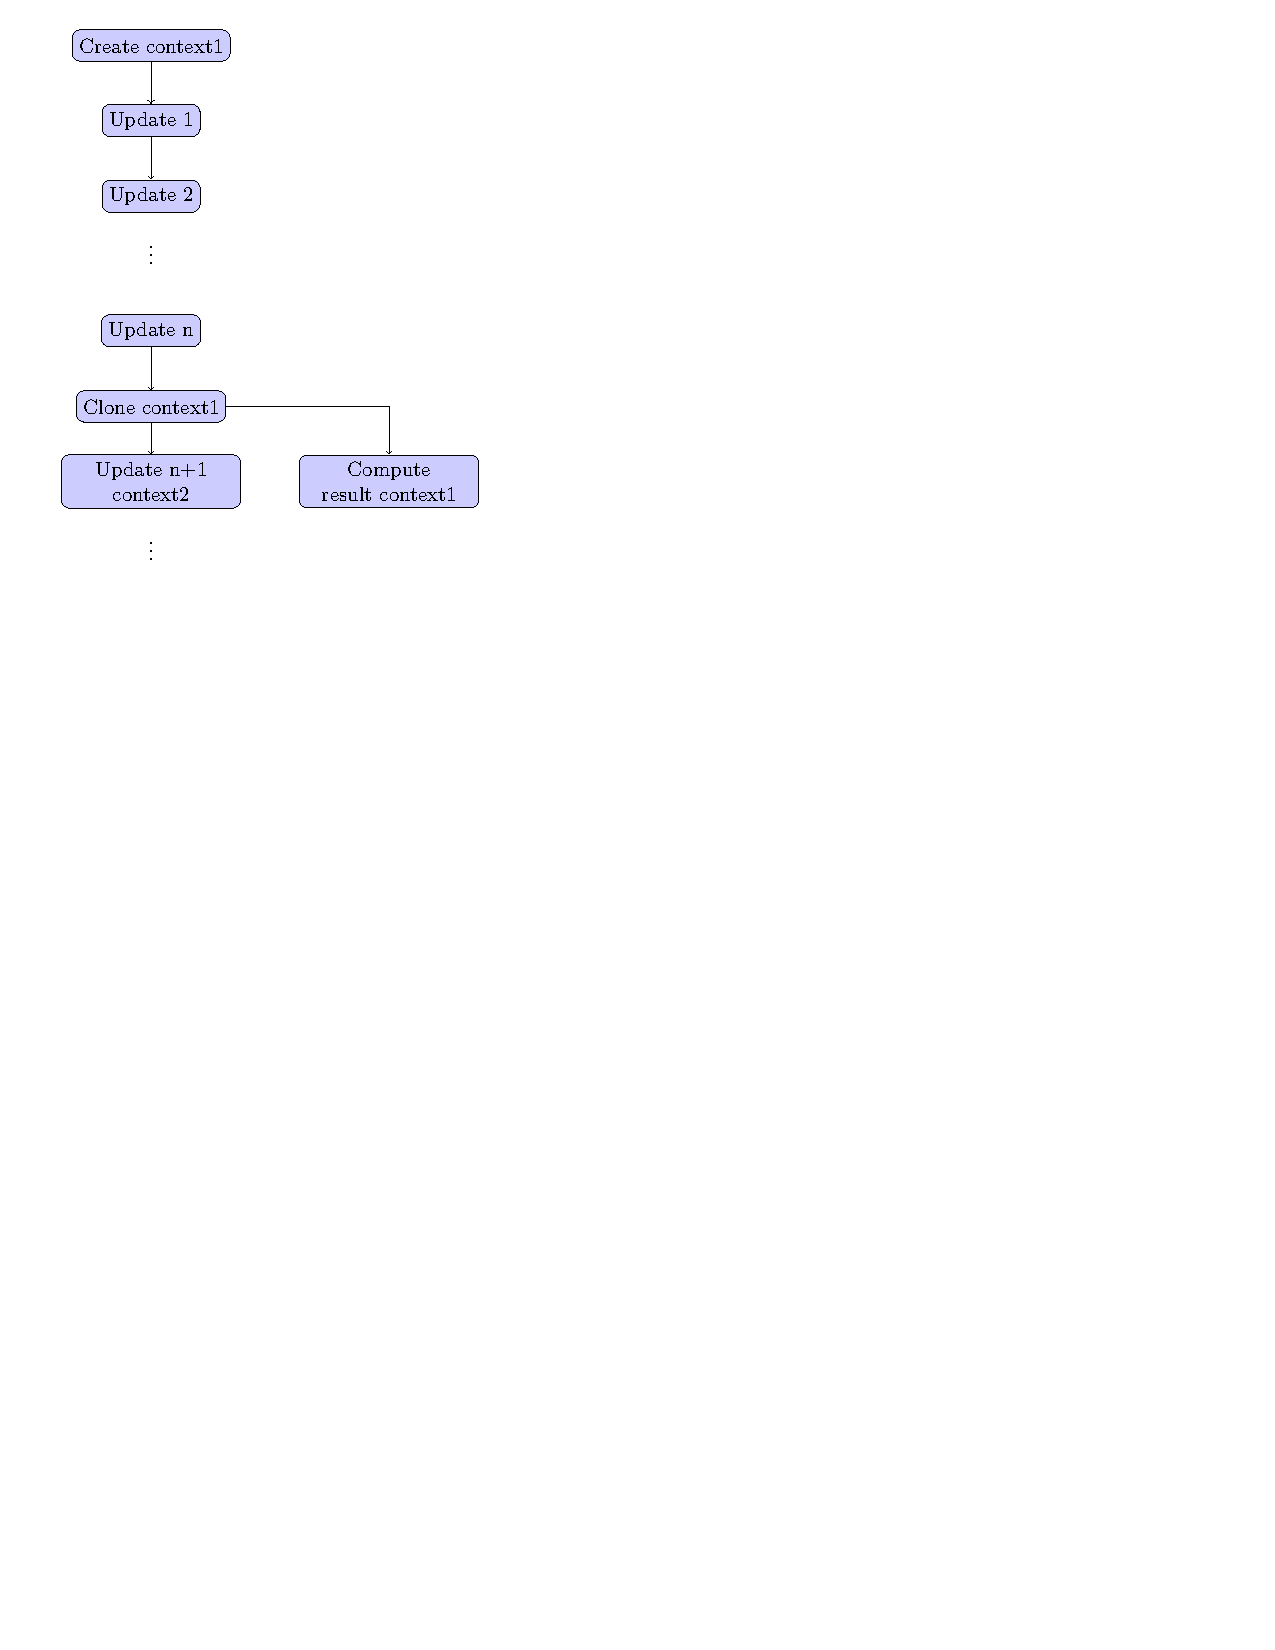
\includegraphics[trim=0cm 18.5cm 9.5cm 0cm,
height=10cm]{figures/hash_signature_clone.pdf}
\caption{Context - clone example\newline}
\label{fig:gci_clone}
%}
\end{figure}
As shown figure \ref{fig:gci_clone}, when we need to compute a result, but the
whole data added previously are needed for a future result, the solution is to
clone the context, meaning that the whole data added and the configuration is copied in another context.\newline
Then one context could be used to compute the result and the other one
to add other data when needed.\newline


\section{Key management}

\label{gci_key_mng}

In the previous version of the \embtls project interacted directly the provider
and the application.
This interaction was used for example to generate and to become directly a key
or to compute something with a key coming from the other peer.
With the interface this is not possible anymore.
That's why the key management is required for the interface.
Through the interface the keys can be saved and used by the provider to compute
something or by the application to send it to another peer.


\subsection*{Put a key}
As said in chapter \ref{gci_gen_key} Generate key pair, when a key is generated,
the ID of the key is returned to the application.
This is because the key is saved in the interface, through the function `` Put
key ``.


\begin{figure}[!ht]
\centering
%\frame{
% trim: left, bottom, right, up
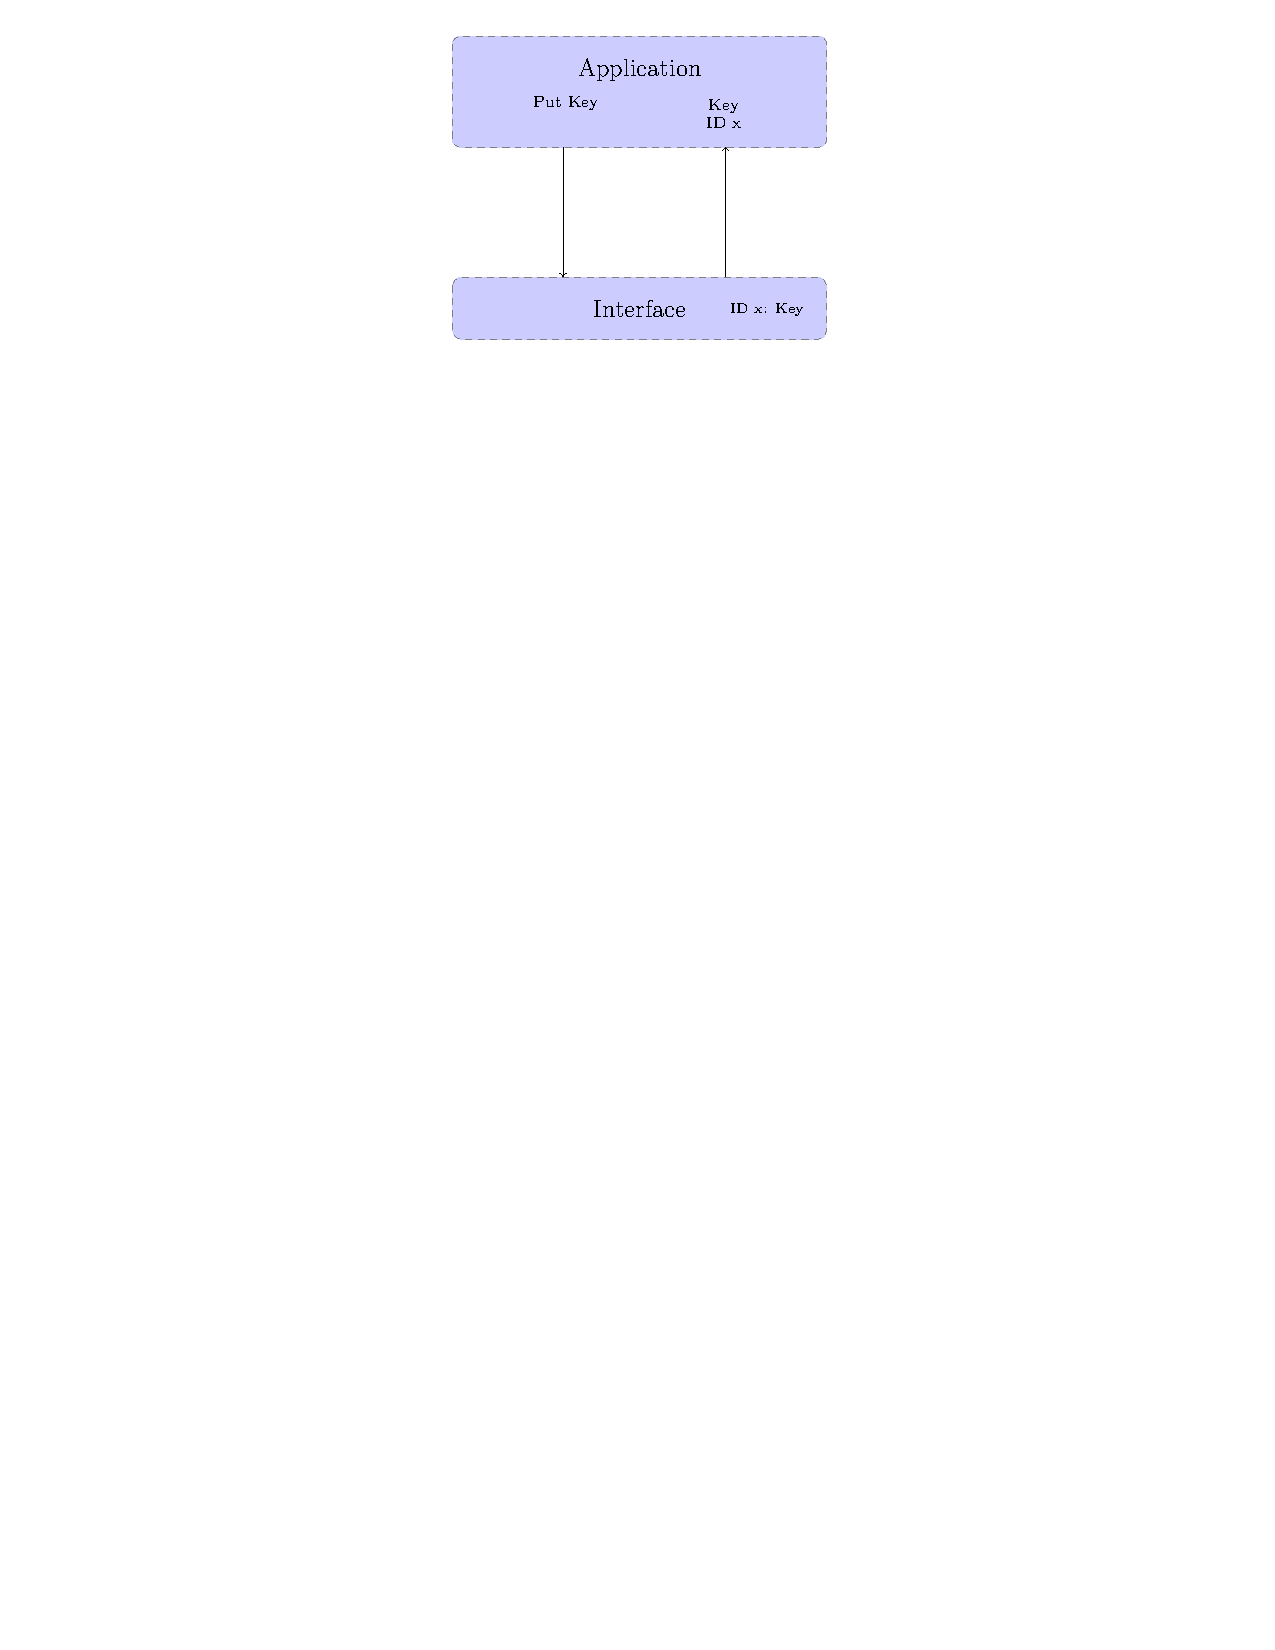
\includegraphics[trim=12cm 22cm 9.5cm 0cm]{figures/key_manag_put_key.pdf}
\caption{Key management - put a key\newline}
\label{fig:gci_key_mng_put}
%}
\end{figure}

As shown on figure \ref{fig:gci_key_mng_put}, when a key should be stored in the
interface, the key is added to the function. The interface saves it in a
specific place and return the ID of where is the key stored.


\subsection*{Get a key}
When the key should be used to be sent to another peer or to compute
something like a signature, it should be possible to get it.

\begin{figure}[!ht]
\centering
%\frame{
% trim: left, bottom, right, up
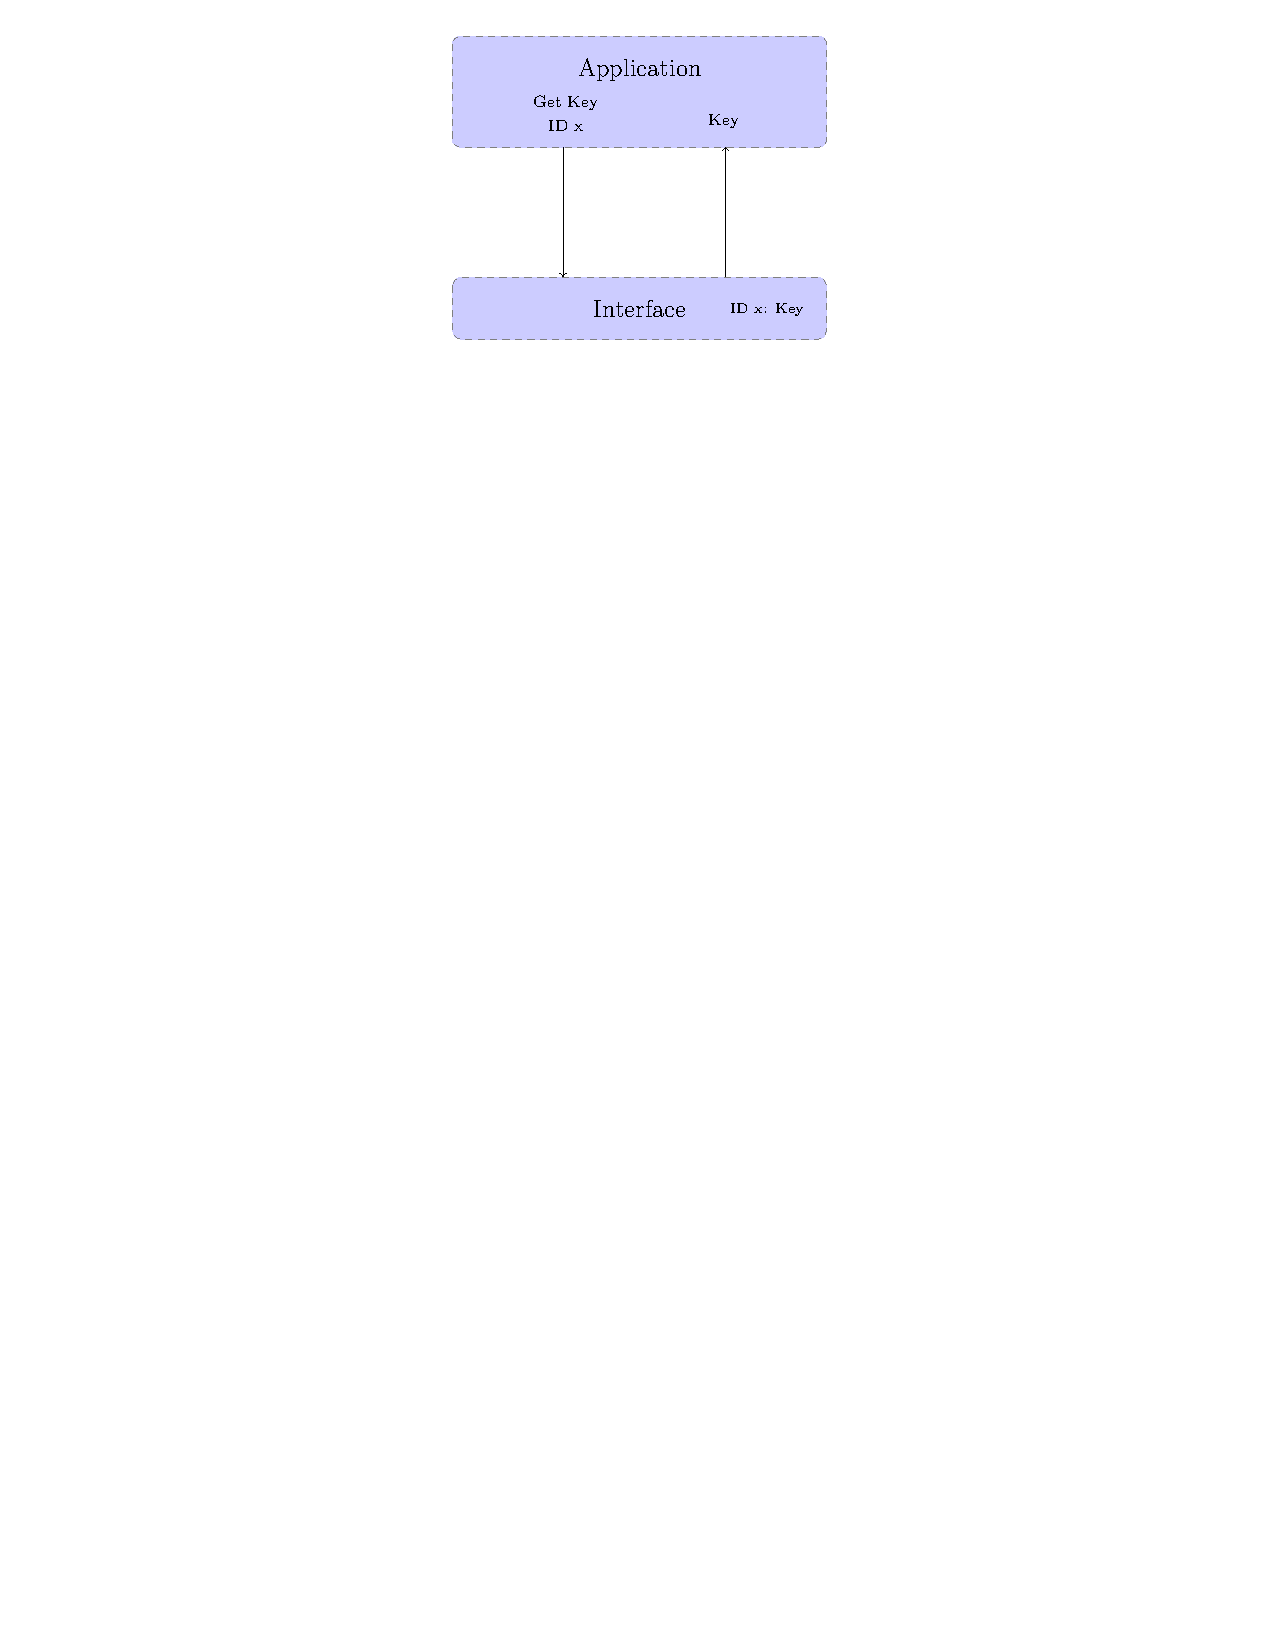
\includegraphics[trim=12cm 22cm 9.5cm 0cm]{figures/key_manag_get_key.pdf}
\caption{Key management - get a key\newline}
\label{fig:gci_key_mng_get}
%}
\end{figure}

As shown on figure \ref{fig:gci_key_mng_get}, when the key is needed by the
application, the ID should be sent the interface which will return the key
stored at this ID.

The key stays in the interface if it's still needed.

\subsection*{Delete a key}
When the key is not needed anymore, it should be possible to delete it to free
space for other keys.

\begin{figure}[!ht]
\centering
%\frame{
% trim: left, bottom, right, up
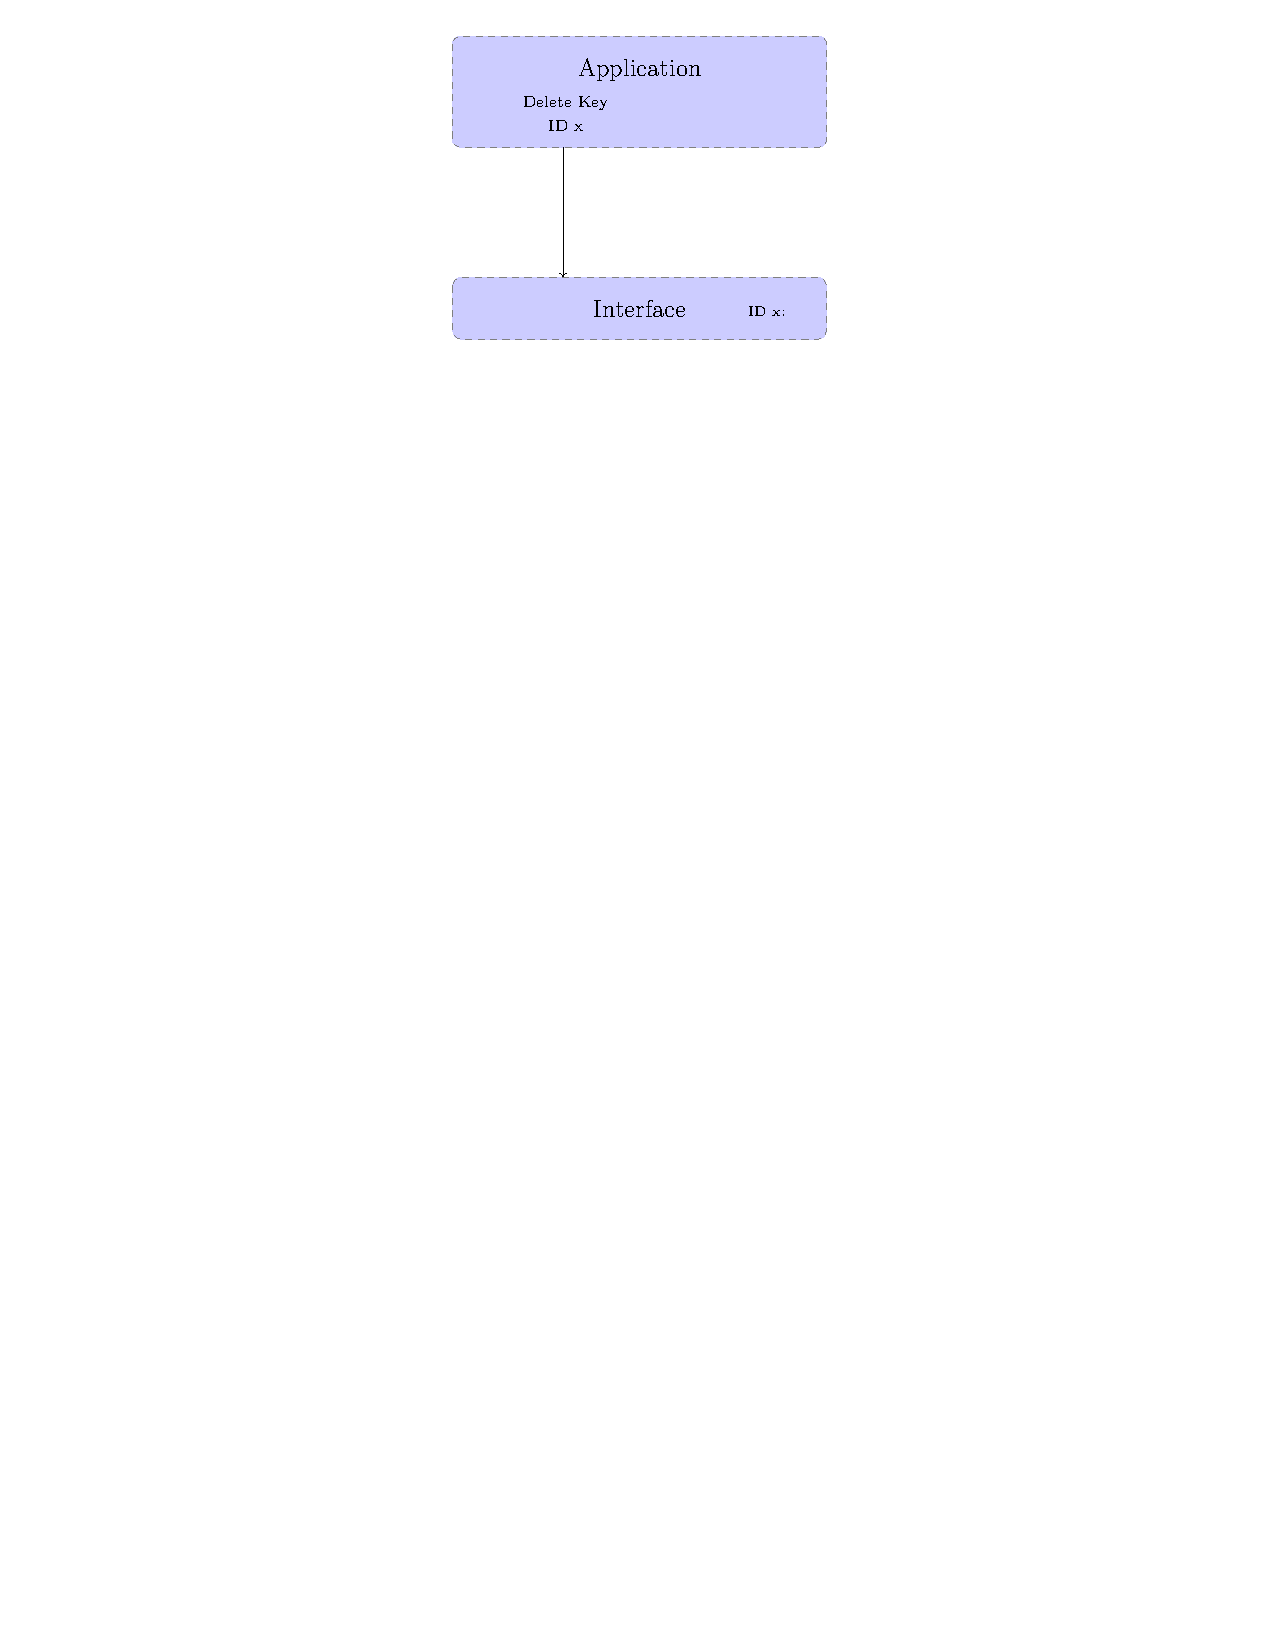
\includegraphics[trim=12cm 22cm 9.5cm 0cm]{figures/key_manag_del_key.pdf}
\caption{Key management - delete a key\newline}
\label{fig:gci_key_mng_del}
%}
\end{figure}

As shown on figure \ref{fig:gci_key_mng_del}, when the key is not needed
anymore, the ID of it is sent to the interface, which will delete it.
